\documentclass[12pt]{article}
\usepackage{amsmath, amssymb, amsthm}
\usepackage{fancyhdr}
\usepackage{lipsum} % for generating dummy text, you can remove this line in your actual document
\usepackage[margin=1in, bottom=1.5in]{geometry} % Adjust bottom margin as needed
\usepackage{thmtools}
\usepackage{listings}
\usepackage{graphicx}
\usepackage{hyperref}

% Page style settings
\pagestyle{fancy}
\fancyhf{} % Clear header and footer
\renewcommand{\headrulewidth}{1pt}
\renewcommand{\footrulewidth}{1pt}
\renewcommand{\labelenumi}{(\alph{enumi})}
\fancyhead[C]{\textbf{\large 1A - Mathematics}}
\fancyfoot[C]{\thepage}

\DeclareMathOperator{\tr}{Tr}

% Macros for convenience
\newcommand{\bbR}{\mathbb{R}} % Example: Real numbers
% Add more macros as needed

\usepackage{mdframed} % For framing
\declaretheoremstyle[
  spaceabove=6pt,
  spacebelow=6pt,
  headfont=\bfseries,
  notefont=\normalfont,
  bodyfont=\normalfont,
  headpunct={},
  postheadspace=1em,
  qed=,
]{mystyle}

\declaretheorem[
  style=mystyle,
  name=Example,
  within=section,
]{example}

% Define a framed theorem environment
\newmdtheoremenv[
  linecolor=black,
  linewidth=1pt,
  topline=true,
  bottomline=true,
  rightline=true,
  leftline=true,
  innertopmargin=10pt,
  innerbottommargin=10pt,
  innerrightmargin=10pt,
  innerleftmargin=10pt
]{proposition}{Proposition}

\newmdtheoremenv[
  linecolor=red,
  linewidth=1pt,
  topline=true,
  bottomline=true,
  rightline=true,
  leftline=true,
  innertopmargin=10pt,
  innerbottommargin=10pt,
  innerrightmargin=10pt,
  innerleftmargin=10pt
]{definition}{Definition}

\newmdtheoremenv[
  linecolor=red,
  linewidth=1pt,
  topline=true,
  bottomline=true,
  rightline=true,
  leftline=true,
  innertopmargin=10pt,
  innerbottommargin=10pt,
  innerrightmargin=10pt,
  innerleftmargin=10pt
]{theorem}{Theorem}
\begin{document}

\title{Engineering Tripos Part IA - Mathematics}
\author{Morărescu Mihnea-Theodor}
\date{\today}

\maketitle

\newpage

\tableofcontents

\newpage

\section{Vectors}

In this section of the course, we will turn our attention to analyzing vectors. We will first being with elements of vector algebra and the various properties of these objects, and then move onto analytic geometry and equations using vectors.

\subsection{Vector algebra}

\begin{definition}[Vector space]
    A vector space over $\mathbb{R}$ or $\mathbb{C}$ is a set $V \neq \emptyset$ with an internal operation (addition), and an external operation (multiplication of a vector with a scalar). 

    Vector addition has to satisfy:

    \begin{enumerate}
        \item $\mathbf{a + b} = \mathbf{b + a}, \forall \mathbf{a, b} \in V$
        \item $(\mathbf{a + b}) + \mathbf{c} = \mathbf{a} + (\mathbf{b + c}), \forall \mathbf{a, b, c} \in V$
        \item There exists an identity element $\mathbf{0} \in V$ so that $\mathbf{a + 0} = \mathbf{0 + a} = \mathbf{a}, \forall \mathbf{a} \in V$
        \item For any vector $\mathbf{a} \in V$, there exists another vector $\mathbf{-a} \in V$ so that $\mathbf{a + (-a)} = \mathbf{(-a) + a} = \mathbf{0}$
    \end{enumerate}

    In other words, $(V, +)$ must be an abelian group. Furthermore, scalar multiplication has to satisfy:

    \begin{enumerate}
        \item $\lambda (\mathbf{a + b}) = \lambda \mathbf{a} + \lambda \mathbf{b}$
        \item $(\lambda + \mu)\mathbf{a} = \lambda\mathbf{a} + \mu\mathbf{a}$
        \item $\lambda(\mu\mathbf{a}) = (\lambda\mu)\mathbf{a}$
        \item $1_{\mathbb{F}}\mathbf{a} = \mathbf{a}$
    \end{enumerate}
\end{definition}

\begin{definition}[Vector]
    For a vector space $V$, we say that any element $\mathbf{v} \in V$ is a vector.
\end{definition}

This is the formal definition of a vector. However, for the sake of keeping things simple, a vector is just a quantity that has both magnitude and direction.

\begin{definition}[Magnitude of a vector]
    Consider a vector $\mathbf{v} \in \mathbb{R}$, with $\mathbf{v} = \begin{bmatrix}
        v_1 \\
        v_2 \\
        \vdots \\
        v_n
    \end{bmatrix}$. We define the magnitude of a vector as:

    \[ \mathbf{|v|} = \sqrt{\sum_{i = 1}^n v_i^2} \]
\end{definition}

\begin{definition}[Unit vector]
    A unit vector $v$ is a vector with unit length (length equal to 1). For any vector $\mathbf{v} \in V$, the unit vector that gives the direction of $\mathbf{v}$ is denoted by $\mathbf{\hat{v}}$ and is given by:

    \[ \mathbf{\hat{v}} = \frac{\mathbf{v}}{|\mathbf{v}|} \]
\end{definition}

\begin{definition}[Vector addition]
    Consider two vectors $\mathbf{v} = \begin{bmatrix}
        v_1 \\
        v_2 \\
        \vdots \\
        v_n
    \end{bmatrix}$ and $\mathbf{u} = \begin{bmatrix}
        u_1 \\
        u_2 \\
        \vdots \\
        u_n
    \end{bmatrix}$. Then, we define the sum of the two vectors as:

    \[ \mathbf{u + v} = \begin{bmatrix}
        u_1 + v_1 \\
        u_2 + v_2 \\
        \vdots \\
        u_n + v_n 
    \end{bmatrix} \]
\end{definition}

\begin{definition}[Scalar product]
    Consider two vectors $\mathbf{v} = \begin{bmatrix}
        v_1 \\
        v_2 \\
        \vdots \\
        v_n
    \end{bmatrix}$ and $\mathbf{u} = \begin{bmatrix}
        u_1 \\
        u_2 \\
        \vdots \\
        u_n
    \end{bmatrix}$. We define the scalar product $\mathbf{u} \cdot \mathbf{v}$ between the two vectors as:

    \[ \mathbf{u} \cdot \mathbf{v} = \mathbf{v} \cdot \mathbf{u} = \sum_{i = 1}^n u_iv_i \]
\end{definition}

Note that the scalar (dot) product is commutative and is also distributive over addition and subtraction. Therefore:

\[ \mathbf{a \cdot b} = \mathbf{b \cdot a} \]
\[  \mathbf{a \cdot (\mathbf{b} + \mathbf{c})} = \mathbf{a \cdot b} + \mathbf{a \cdot c} \]

However, sometimes we might be interested in finding the scalar product between two vectors, yet we only have information about their magnitudes and the angle between them - how would we proceed in this case?

\begin{proposition}[Magnitude using scalar product]
    The magnitude of a vector $\mathbf{v} \in V$ can be expressed, using the scalar product, as:

    \[ \mathbf{|v|^2} = \mathbf{v \cdot v} \]
\end{proposition}

\begin{theorem}[Scalar product equivalence]
    Consider two vectors $\mathbf{a, b} \in \mathbb{R}^3$. Their scalar product is given by:

    \[ \mathbf{a \cdot b} = \mathbf{|a||b|}\cos{\theta} \]

    Where $\theta$ is the angle between $\mathbf{a}$ and $\mathbf{b}$.
\end{theorem}

\begin{proof}
    Consider two points in space with position vectors $\mathbf{a}$ and $\mathbf{b}$. We define $\mathbf{c = a - b}$. Therefore:

    \[ \mathbf{|c|}^2 = \mathbf{(a - b) \cdot (a - b)} = \mathbf{a \cdot a - a \cdot b - b \cdot a + b \cdot b} = \mathbf{|a|^2 + |b|^2} - 2\mathbf{a \cdot b } \]

    However, from the cosine rule, we obtain:

    \[ \mathbf{|c|}^2 = \mathbf{|a|^2 + |b|^2} - 2\mathbf{|a||b|}\cos{\theta} \]

    Hence, $\mathbf{a \cdot b} = \mathbf{|a||b|}\cos{\theta}$.
\end{proof}

\begin{proposition}[Angle between two vectors]
    For any two vectors $\mathbf{x, y} \in \mathbb{R}^n$, we can define the angle between the two vectors as:

    \[ \cos{\theta} = \frac{\mathbf{x \cdot y}}{\mathbf{|x||y|}} \]
\end{proposition}

\begin{definition}[Vector product]
    Consider two vectors $\mathbf{a, b} \in \mathbb{R}^3$. We define the vector product between them as:

    \[ \mathbf{a} \times \mathbf{b} = \begin{vmatrix}
        \mathbf{i} && \mathbf{j} && \mathbf{k} \\
        a_x && a_y && a_z \\
        b_a && b_y && b_z
    \end{vmatrix} \]
\end{definition}

Using the properties of the determinant, from the definition it follows that:

\[ \mathbf{a \times b = - b \times a} \]

Hence, the vector product is anti-commutative. Moreover, by setting $\mathbf{b} \to \mathbf{a}$, we obtain:

\[ \mathbf{a \times a} = - \mathbf{a \times a} \Leftrightarrow \mathbf{a \times a} = \mathbf{0} \]

Note that the vector product between $\mathbf{a}$ and $\mathbf{b}$ returns a vector $\mathbf{c}$ that is perpendicular to both $\mathbf{a}$ and $\mathbf{b}$.

\begin{theorem}[Magnitude of the vector product]
    For any two vectors $\mathbf{a, b} \in \mathbb{R}^3$, the magnitude of their vector product is given by:

    \[ |\mathbf{a \times b}| = \mathbf{|a||b|}\sin{\theta} \]

    Where $\theta$ is the angle between the two vectors. Also note that the vector product can only be defined in $\mathbb{R}^3$ (it cannot be generalized for higher dimensions).
\end{theorem}

\begin{definition}[Basis]
    Let $V \neq \emptyset$ be a vector space. We say that $B = \{\mathbf{e_1}, \dots, \mathbf{e_n}\}$ is a basis if every element of $V$ can be written as a linear combination of the elements of $B$, i.e. $\forall \mathbf{v} \in V$, $\exists \alpha_1, \dots, \alpha_n \in K$ (the field over which we defined the external operation), such that:

    \[ \mathbf{v} = \sum_{i = 1}^n \alpha_i \mathbf{e_i} \]
\end{definition}

\begin{definition}[Linear independence]
    Let $V \neq \emptyset$ be a vector space. We say that any vectors $\mathbf{v_1, v_2, \dots, v_n}$ are linearly independent if $\forall \lambda_1, \lambda_2, \dots, \lambda_n \in K$, then:

    \[ \sum_{i = 1}^n \lambda_i\mathbf{v_i} = \mathbf{0} \iff \lambda_i = 0, \forall 1 \leq i \leq n \]
\end{definition}

\begin{theorem}[Generating bases in $\mathbb{R}^3$]
    Consider two vectors $\mathbf{a, b} \in \mathbb{R}^3$ such that $\mathbf{a \times b} \neq \mathbf{0}$. Then, the set $B = \{\mathbf{a, b, a \times b}\}$ forms a basis of $\mathbb{R}^3$. (Note that this is true provided the two vectors are not parallel).
\end{theorem}

Therefore, $\forall \mathbf{x} \in \mathbb{R}^3, \exists \alpha, \beta, \gamma \in \mathbb{R}$ so that:

\[ \mathbf{x} = \alpha\mathbf{a} + \beta\mathbf{b} + \gamma\mathbf{a \times b} \]

\begin{definition}[Scalar triple product]
    Consider three arbitrary vectors $\mathbf{a, b, c} \in \mathbb{R}^3$. We define the scalar triple product between the vectors as:

    \[ [\mathbf{a, b, c}] = \mathbf{a \cdot (\mathbf{b \times c})}\] 
\end{definition}

The geometrical interpretation of the scalar triple product is that it is equal to the volume of the parallelepiped formed by the three vectors.

\begin{proposition}[Properties of the scalar triple product]
    Consider three vectors $\mathbf{a, b, c} \in \mathbb{R}^3$. Then:

    \begin{enumerate}
        \item $\mathbf{a \cdot (b \times c)} = \mathbf{b \cdot (c \times a)} = \mathbf{c \cdot (a \times b)} = [\mathbf{a, b, c}]$ (Cyclic property)
        \item $\mathbf{a \cdot (b \times c)} = \mathbf{(a \times b) \cdot c}$ (We can replace the dot with the cross)
        \item If all vectors are co-planar, then $\mathbf{[a, b, c]}$ = 0
        \item If $\mathbf{[a, b, c]} > 0$, the three vectors form a right-handed set. Otherwise, they form a left-handed set.
        \item $\mathbf{[a, b, c]} = \begin{vmatrix}
            a_x & a_y & a_z \\
            b_x & b_y & b_z \\
            c_x & c_y & c_z
        \end{vmatrix}$
        \item $\forall \lambda \in \mathbb{R}, [\lambda\mathbf{a, b, c}] = \lambda[\mathbf{a, b, c}]$
    \end{enumerate}
\end{proposition}

\begin{definition}[Vector triple product]
    Consider three vectors $\mathbf{a, b, c} \in \mathbb{R}^3$. We define the vector triple product between these vectors as:

    \[ \mathbf{a \times (b \times c)} = (\mathbf{a \cdot c})\mathbf{b} - (\mathbf{a \cdot b})\mathbf{c} \]
    \[ (\mathbf{a \times b}) \times \mathbf{c} = (\mathbf{a \cdot c})\mathbf{b} - (\mathbf{b \cdot c})\mathbf{a} \]
\end{definition}

\newpage

\subsection{Analytic geometry in $\mathbb{R}^3$}

\begin{proposition}[Equation of line]
    Consider a line which contains a point with position vector $\mathbf{a}$ and direction vector given by $\mathbf{b}$. The equation of the line is then given by:

    \[ \mathbf{r} = \mathbf{a} + \lambda\mathbf{b}, \lambda \in \mathbb{R} \]

    The proof is trivial.
\end{proposition}

\begin{proposition}[Cartesian equivalent of line equation I]
    Consider a line given by $\mathbf{r} = \mathbf{a} + \lambda \mathbf{b}$. Then, the equation of this line in Cartesian form is given by:

    \[ \frac{x - a_x}{b_x} = \frac{y - a_y}{b_y} = \frac{z - a_z}{b_z} \]
\end{proposition}

\begin{proof}
    We can rewrite the equation of line using matrix form as:

    \[ \begin{bmatrix}
        x \\
        y \\
        z
    \end{bmatrix} = \begin{bmatrix}
        a_x \\
        a_y \\
        a_z
    \end{bmatrix} + \lambda \begin{bmatrix}
        b_x \\
        b_y \\
        b_z
    \end{bmatrix} \]

    Therefore, $x = a_x + \lambda b_x$, $y = a_y + \lambda b_y$ and $z = a_z + \lambda b_z$. Note that this is also known as the parametric form of the line equation, where every component is expressed in terms of a parameter $\lambda$. By expressing $\lambda$ for each one of these, we obtain the conclusion. 
\end{proof}

Note that in order to obtain different points on a line, we need to vary $\lambda$.

\begin{proposition}[Equation of line between two points]
    Consider two points with position vectors $\mathbf{a, b} \in \mathbb{R}^3$. Therefore, the line between these two points is given by:

    \[ \mathbf{r} = \mathbf{a} + \lambda (\mathbf{b - a}) \]
\end{proposition}

The conclusion follows because we can take $\mathbf{b - a}$ to be the direction vector of the line.

\begin{proposition}[Cartesian equivalent of line equation II]
    Consider a line given by $\mathbf{r} = \mathbf{a} + \lambda \mathbf{(b - a)}$. Then, the equation of this line in Cartesian form is given by:

    \[ \frac{x - a_x}{b_x - a_x} = \frac{y - a_y}{b_y - a_y} = \frac{z - a_z}{b_z - a_z} \]
\end{proposition}

\begin{proposition}[Second form of an equation of a line]
    Consider a line given by $\mathbf{r} = \mathbf{a} + \lambda\mathbf{b}$. By considering $\mathbf{b \times r}$, we obtain:

    \[ \mathbf{b \times r} = \mathbf{b \times a} \]

    By defining a new vector $\mathbf{c} = \mathbf{b \times a}$, we obtain the second form of a line equation:

    \[ \mathbf{b \times r} = \mathbf{c} \]
\end{proposition}

\begin{proposition}[Intersection between two lines]
    Consider two lines given by $\mathbf{r_1} = \mathbf{a_1} + \lambda_1\mathbf{b_1}$ and $\mathbf{r_2} = \mathbf{a_2} + \lambda_2\mathbf{b_2}$. We want to determine the intersection point between these two lines. Therefore, we begin by parametrizing the line as: $x_1(\lambda_1) = a_{1_x} + \lambda_1b_{1_x}$, $x_2(\lambda_2) = a_{2_x} + \lambda_2b_{2_x}$, and $y_1(\lambda_1) = a_{1_y} + \lambda_1b_{1_y}$, $y_2(\lambda_2) = a_{2_y} + \lambda_2b_{2_y}$. We then determine $\lambda_1, \lambda_2$ so that $x_1 = x_2$ and $y_1 = y_2$, and afterwards we might perform a sanity check to make sure that $z_1 = z_2$.
\end{proposition}

\begin{proposition}[Distance between point and line]
    Consider a line given by $\mathbf{r} = \mathbf{a} + \lambda\mathbf{b}$ and a point with position vector $\mathbf{p}$. The distance between the point $P$ and the line is given by:

    \[ \delta = \frac{|(\mathbf{p - a}) \times \mathbf{b}|}{|\mathbf{b}|} \]
\end{proposition}

\begin{proof}
        Consider the angle given between the line $AP$ and the direction vector $\mathbf{b}$. We observe that $\sin{\theta} = \frac{\delta}{\mathbf{|p - a|}}$. Therefore, $\delta = |\mathbf{p - a}|\sin{\theta}$. We can then express the sine term as:

        \[ \delta = \frac{|(\mathbf{p - a}) \times \mathbf{b}|}{|\mathbf{b}|} \]

        Thus concluding the proof.
    \end{proof}

Note that if we have to find the distance between two parallel lines, the problem is equivalent to finding the distance between any point on one line to the second line.

\begin{proposition}[Distance between two skew lines]
    Consider two skew lines given by equations $\mathbf{r_1} = \mathbf{a_1} + \lambda\mathbf{b_1}$ and $\mathbf{r_2} = \mathbf{a_2} + \mu\mathbf{b_2}$. Therefore, the distance between the two lines is given by:

    \[ \delta = \frac{|(\mathbf{a_2 - a_1})\cdot(\mathbf{b_1 \times b_2})|}{|\mathbf{b_1 \times b_2}|} \]
\end{proposition}

\begin{proof}
    We first being by determining a vector that is perpendicular to both lines. This is given by:

    \[ \mathbf{n} = \mathbf{b_1 \times b_2} \]

    We do not want to alter, however, the length of our distance. For this reason, we normalize this vector, and we obtain:

    \[ \mathbf{\dot{n}} = \frac{\mathbf{b_1 \times b_2}}{|\mathbf{b_1 \times b_2}|} \]

    Hence, the distance between the two lines is given by the component in the direction of $\mathbf{\dot{n}}$ of $\mathbf{r_2 - r_1}$. We are then free to pick any two points on the line, hence:

    \[ \delta = |\mathbf{(r_2 - r_1) \cdot \dot{n}}| = \frac{|(\mathbf{a_2 - a_1})\cdot(\mathbf{b_1 \times b_2})|}{|\mathbf{b_1 \times b_2}|} \]
\end{proof}

\begin{proposition}[Equation of plane]
    Consider a plane $\Pi$, a point $A \in \Pi$ with position vector $\mathbf{a}$, and a vector $\mathbf{n}$ that is normal to the plane. Therefore, the equation of the plane is:

    \[ \mathbf{(r - a) \cdot n} = 0 \]

    The geometrical meaning is extremely intuitive: the equation above just tells us that the plane represents the set of points in space for which the line $AP$ is perpendicular to $\mathbf{n}$.
\end{proposition}

This equation can be rearranged into:

\[ \mathbf{r \cdot n - a \cdot n} = 0 \Leftrightarrow \mathbf{r \cdot n = a \cdot n} \]

By denoting $d = \mathbf{a \cdot n}$ (note that this is the distance from the origin to the plane), we obtain a simplified version of the plane equation:

\[ \mathbf{r \cdot n} = d \]

\begin{proposition}[Cartesian equation of plane]
    Consider a plane given by $\mathbf{r \cdot n} = d$. The equation in Cartesian coordinates is given by:

    \[ ax + by + cz = d \]

    Where $\mathbf{n} = \begin{bmatrix}
        a \\
        b \\
        c
    \end{bmatrix}$. By setting $d \to -d$, we can obtain an equivalent expression:

    \[ ax + by + cz + d = 0 \]
\end{proposition}

\begin{proposition}[Equation of plane between three points]
    Consider three points $A, B, C$ in space with position vector $\mathbf{a, b, c}$. We can obtain the expression of the plane determined by these three points by either considering the normal vector $\mathbf{n} = (\mathbf{b - a}) \times (\mathbf{c - a})$ and then we obtain $\mathbf{(r - a)\cdot n} = 0$, or by considering:

    \[ \mathbf{r} = \mathbf{a} + \lambda\mathbf{(b - a)} + \mu\mathbf{(c - a)} \]

    This is equivalent to:

    \[ \mathbf{r} = (1 - \lambda - \mu)\mathbf{a} + \lambda\mathbf{b} + \mu\mathbf{c} \]

    By setting $\alpha = 1 - \lambda - \mu$, $\beta = \lambda$ and $\gamma = \mu$, we obtain the equivalent plane equation:

    \[ \mathbf{r} = \alpha\mathbf{a} + \beta\mathbf{b} + \gamma\mathbf{c}, \alpha + \beta + \gamma = 1 \]
\end{proposition}

\begin{proposition}[Distance between point and plane]
    Consider a point $P(x_0, y_0, z_0) \in \mathbb{R}^3$ and a plane given by $\mathbf{r \cdot n} = d$ and normal vector given by $\mathbf{n} = \begin{bmatrix}
        a \\
        b \\
        c
    \end{bmatrix}$, the distance between $P$ and the plane is:

    \[ \delta = \frac{|ax_0 + by_0 + cz_0 + d|}{\sqrt{a^2 + b^2 + c^2}} \]
\end{proposition}

Note that if we have to calculate the distance between a line and a plane, we distinguish between two cases:

\begin{enumerate}
    \item If the line and the plane are not parallel, then they intersect, and therefore the distance is null
    \item If the line and the plane are parallel, the problem is equivalent to obtaining the coordinates of a point on the line and calculating the distance from said point to the plane
\end{enumerate}

\begin{proposition}[Intersection between a line and a plane]
    Consider a line given by $\mathbf{r} = \mathbf{a} + \lambda\mathbf{b}$ and a plane given by $\mathbf{r} \cdot \mathbf{n} = d$. In order to find the intersection between a line and a plane, we need to proceed as follows:

    \begin{enumerate}
        \item Parametrize the line by expressing $x = x(\lambda), y = y(\lambda)$ and $z = z(\lambda)$
        \item Express the plane in Cartesian form as $ax + by + cz + d = 0$
        \item By using the parametrization above, use the equation of the plane and determine $\lambda$
        \item We distinguish between three cases: (i) if we have a unique solution, then we have a point of intersection, (ii) if we obtain a truism (i.e. 0 = 0), the line is contained within the plane, (iii) if we obtain a false expression, then the line and the plane do not intersect
    \end{enumerate}
\end{proposition}

\begin{proposition}[Intersection between three planes]
    Consider two planes given by the equations $\mathbf{r_1 \cdot n_1} = d_1$ and $\mathbf{r_2 \cdot n_2} = d_2$. The general procedure for determining the intersection between the planes is:

    \begin{enumerate}
        \item Derive the Cartesian equations for both planes, i.e. $a_1x + b_1y + c_1z + d_1 = 0$ and $a_2x + b_2y + c_2z + d_2 = 0$
        \item Solve the given system of equations (which has either no solution or infinitely many solutions)
        \item If the system has no solutions, the planes are parallel. Otherwise, the intersection of the two planes is a line
    \end{enumerate}
\end{proposition}

\newpage

\subsection{Vector equations}

The general strategy when solving vector equations is to either take the scalar or vector product of the equation with suitable vectors in order to further reduce it. Otherwise, if we cannot perform this simplification or after the equation has been sufficiently simplified, we can write component-wise equations.

\begin{example}
    Simplify the following vector equation: $\mathbf{x} - (\mathbf{x \times a}) \times \mathbf{b} = \mathbf{c}$. 

    The equation can be expanded using the triple vector product as:

    \[ \mathbf{x} - (\mathbf{x \cdot b})\mathbf{a} + (\mathbf{a} \cdot \mathbf{b})\mathbf{x} = \mathbf{c} \]

    We can dot the above equation with $\mathbf{b}$ to obtain:

    \[ \mathbf{x \cdot b} - (\mathbf{x} \cdot \mathbf{b})(\mathbf{a} \cdot \mathbf{b}) + (\mathbf{a} \cdot \mathbf{b})(\mathbf{x} \cdot \mathbf{b}) = \mathbf{c \cdot b} \]

    Which can be further simplified to:

    \[ \mathbf{x \cdot b} = \mathbf{c \cdot b} \]
\end{example}

\newpage

\section{Functions and series approximation}

In this section we are concerned with curve sketching, performing revision of functions and extending some concepts.

\subsection{Curve sketching}

\begin{definition}[Even function]
    We say that a function $f : \mathbb{R} \to \mathbb{R}$ is even if $\forall x \in \mathbb{R}, f(-x) = f(x)$.
\end{definition}

\begin{definition}[Odd function]
    We say that a function $f : \mathbb{R} \to \mathbb{R}$ is odd if $\forall x \in \mathbb{R}, f(-x) = -f(x)$.
\end{definition}

\begin{theorem}
    Any function $f : \mathbb{R} \to \mathbb{R}$ can be written as the sum of an even and an odd function.
\end{theorem}

\begin{proof}
    Choose $g, h : \mathbb{R} \to \mathbb{R}$, with $g(x) = \frac{f(x) + f(-x)}{2}$ and $h(x) = \frac{f(x) - f(-x)}{2}$. Then, $g(x)$ is an even function, while $h(x)$ is odd, and then:

    \[ f(x) = g(x) + h(x), \forall x \in \mathbb{R} \]
\end{proof}

\begin{theorem}
    Let $f : \mathbb{R} \to \mathbb{R}$ be a differentiable function. If $f$ is odd, then $f(0) = 0$. If $f$ is even, then $f'(0) = 0$.
\end{theorem}

We will now consider a general algorithm to follow whenever sketching curves.

\begin{enumerate}
    \item Solve the equation $f(x) = 0$ and find the intersection points with the $Ox$ axis
    \item Find the intersection with the $Oy$ axis, i.e. $f(0)$
    \item Take the limits at the extreme points of the domain, i.e. $\lim_{x \to \pm \infty} f(x)$ or otherwise
    \item Determine all the points of discontinuity (singularities)
    \item Determine $f'(x)$ and set $f'(x) = 0$ and determine the monotonicity intervals. Note that $f'(x) \geq 0$ implies function is increasing, and $f'(x) \leq 0$ implies function is decreasing. Note that for a point $x_0 \in \mathbb{R}$, if $f'(x_0) \geq 0, \forall x \geq x_0$ and $f'(x_0) \leq 0, \forall x \leq x_0$, then $x_0$ is a minima. If the inverse is true, then it is a point of maxima.
    \item Determine $f''(x)$ and determine the function's convexity intervals
    \item Sketch the curve
\end{enumerate}

\newpage

\subsection{Hyperbolic functions}

The hyperbolic functions are functions expressed in terms of exponentials, that are closely related to the trigonometric functions. We will further explore this relationship in the next chapter, where we will thoroughly analyze complex numbers.

\begin{definition}[Hyperbolic functions]
    We define the hyperbolic sine and cosine as $\sinh, \cosh : \mathbb{R} \to \mathbb{R}$, with:

    \[ \sinh{x} = \frac{e^x - e^{-x}}{2}, \cosh{x} = \frac{e^x + e^{-x}}{2} \]
\end{definition}

From the above definition, we can easily deduce the hyperbolic tangent (and respectively the hyperbolic cotangent):

\[ \tanh{x} = \frac{e^x - e^{-x}}{e^x + e^{-x}} \]

Furthermore, by differentiating the hyperbolic functions, we obtain that $\sinh'(x) = \cosh{x}$ and $\cosh'(x) = \sinh{x}$. These appear similar to the normal trigonometric functions, however we must note that the derivative of the hyperbolic cosine does not contain a minus sign. Furthermore, $\tanh'(x) = \frac{1}{\cosh^2{x}}$.

Below, we will list some important identities of the hyperbolic functions:

\begin{enumerate}
    \item $\sinh{x} + \cosh{x} = e^x, \forall x \in \mathbb{R}$
    \item $\cosh{x} - \sinh{x} = e^{-x}, \forall x \in \mathbb{R}$
    \item $\cosh^2{x} + \sinh^2{x} = 1, \forall x \in \mathbb{R}$
\end{enumerate}

We will prove the usual trigonometric identities in the complex numbers section of this course.

\begin{example}[Inverse hyperbolic sine]
    Compute $\sinh^{-1}{x}$.
    Let $y = \sinh{x}$. Therefore, $y = \frac{e^x - e^{-x}}{2}$, and by expanding this relationship, we obtain:

    \[ e^x - 2y - e^{-x} = 0 \]

    Multiplying the above by $e^x$ (note that $e^x > 0, \forall x \in \mathbb{R}$), we obtain:

    \[ e^{2x} - 2ye^x - 1 = 0 \]

    This is a quadratic equation in $x$, and we can simply proceed as per usual to obtain an expression for $e^x$. The discriminant is then $\Delta = 4y^2 + 4$, and therefore:

    \[ e^x = y \pm \sqrt{y^2 + 1} \]

    Because $e^x > 0, \forall x \in \mathbb{R}$ and because $\sqrt{x^2 + 1} > x, \forall x \in \mathbb{R}$, we can only allow for the positive solution. Therefore:

    \[ x = \ln{(y + \sqrt{y^2 + 1})} \]

    And therefore we obtain:

    \[ \sinh^{-1}{x} = \ln{(x + \sqrt{x^2 + 1})} \]
\end{example}

We can proceed in a similar fashion to obtain expressions for the inverse hyperbolic cosine and tangent.

\newpage

\subsection{Taylor series expansion}

\begin{theorem}[Taylor series]
    Consider an indefinitely differentiable function $f : \mathbb{R} \to \mathbb{R}$. The Taylor expansion of $f(x)$ about a point $x_0 \in \mathbb{R}$ is given by:

    \[ f(x) = f(x_0) + \sum_{n = 1}^\infty \frac{f^{(n)}(x_0)(x - x_0)^n}{n!} \]
\end{theorem}

\begin{proof}
    The Taylor series expansion can be proved by considering a polynomial expansion of $f(x)$ of the form:

    \[ f(x) = \sum_{n = 0}^\infty \alpha_n(x - x_0)^n \]

    Setting $x \to x_0$, we obtain that $\alpha_0 = f(x_0)$. By differentiating once and setting $x \to x_0$ again, we obtain $\alpha_1 = f'(x_0)$. In general, by differentiating $n$ times and setting $x \to x_0$, we obtain:

    \[ \alpha_n = \frac{f^{(n)}(x_0)}{n!} \]
\end{proof}

\begin{definition}[Maclaurin series]
    The Maclaurin series of a function $f : \mathbb{R} \to \mathbb{R}$ is given by the Taylor series expansion of the function about $x_0 = 0$, i.e.:

    \[ f(x) = \sum_{n = 0}^\infty \frac{f^{(n)}(0)}{n!}x^n \]
\end{definition}

Sometimes, it is useful to expand the Taylor polynomial up until a certain power $k \in \mathbb{N}$, and ignore the other terms. This is called the big $O$ notation, and we usually denote the remainder as:

\[ f(x) =  \sum_{n = 0}^k \frac{f^{(n)}(x_0)(x - x_0)^n}{n!} + \mathcal{O}(x^{k + 1}) \]

This effectively means that $\mathcal{O}(x^{k+1}) \to 0$, or that all the terms above the power $k$ can be neglected. Also note that:

\begin{enumerate}
    \item $\mathcal{O}(x^m) + \mathcal{O}(x^n) = \mathcal{O}(x^d)$, where $d = \min{(m, n)}$
    \item $\mathcal{O}(x^m)\mathcal{O}(x^n) = \mathcal{O}(x^{m + n})$
\end{enumerate}

\begin{example}[Maclaurin series for usual functions]
    Below, we list a few usually encountered functions and their Maclaurin expansion:

    \begin{enumerate}
        \item $e^x = \sum_{n = 0}^\infty \frac{x^n}{n!}$
        \item $\sin{x} = x - \frac{x^3}{3!} + \frac{x^5}{5!} + \dots$
        \item $\cos{x} = 1 - \frac{x^2}{2!} + \frac{x^4}{4!} + \dots$
        \item $(1 + x)^\alpha = 1 + \alpha x + \frac{\alpha (\alpha - 1)}{2!}x^2 + \dots$
        \item $\ln{(1 + x)} = x - \frac{x^2}{2} + \frac{x^3}{3} + \dots$
    \end{enumerate}
\end{example}

\begin{proposition}[Gamma factorial]
    The factorial function can be extended to the real and complex numbers by the function:

    \[ \Gamma(x) = \int_0^\infty t^{x-1}e^{-t}dt \]

    Note that $\Gamma(n) = (n-1)!, \forall n \in \mathbb{N}$.
\end{proposition}

\begin{proposition}[Stirling's approximation]
    For any $n \in \mathbb{N}$, the value of $n!$ can be approximated by:

    \[ n! \approx \left(\frac{n}{e}\right)^n\sqrt{2n\pi} \]
\end{proposition}

\begin{theorem}[L'Hôpital's rule]
    Let $I \subset \mathbb{R}$ and $f,g : I \to \mathbb{R}$ be two differentiable functions on $I \setminus \{x_0\}$, with $\lim_{x \to x_0} f(x) = \lim_{x \to x_0} g(x) = 0$ or $\pm \infty$ and $g'(x) \neq 0, \forall x \in I \setminus \{x_0\}$. Then:

    \[ \lim_{x \to x_0} \frac{f(x)}{g(x)} = \lim_{x \to x_0} \frac{f'(x)}{g'(x)} \]
\end{theorem}

\newpage

\section{Complex numbers}

In this section of the course, we are concerned with studying complex numbers and their various applications within multiple areas of Engineering.

\subsection{The Argand plane}

\begin{definition}[Complex number]
    A complex number $z \in \mathbb{C}$ can be represented as $z = a + bi$, where $a, b \in \mathbb{R}$ and $i$ is defined as $i^2 = -1$.
\end{definition}

\begin{definition}[Modulus of a complex number]
    The modulus of a complex number $z \in \mathbb{C}, z = a + bi, a, b \in \mathbb{R}$ is defined as:

    \[ |z| = \sqrt{a^2 + b^2} \]
\end{definition}

\begin{definition}[Complex conjugate]
    Let $z \in \mathbb{C}$. The complex conjugate $\overline{z}$ is defined as $\overline{z} = a - bi$, where $z = a + bi$.
\end{definition}

Note the useful property that $z\overline{z} = |z|^2$.

\begin{proposition}[Trigonometric form of a complex number]
    Any complex number $z \in \mathbb{C}$ can be represented in trigonometric form as:

    \[ z = r(\cos{\theta} + i\sin{\theta}) \]

    Where $r = |z| = \sqrt{a^2 + b^2}$ and $\tan{\theta} = \frac{b}{a}$. Note that $\theta$ is also called the argument of $z$, and is denoted by $\arg{z} = \theta$.
\end{proposition}

Curves in the complex plane can be defined by the locus of points that satisfy a certain relationship. To determine the loci, we always let $z = x + iy$ and rearrange the given equation to determine its Cartesian equation.

\begin{example}
    Determine the loci $|z+2| = 2|z-1|$.

    Let $z \in \mathbb{C}$, with $z = x + iy$. Then, the equation becomes:
    
    \[ |z+2|^2 = 4|z-1|^2 \Leftrightarrow \]
    \[ |(x+2) + iy|^2 = 4|(x-1) + iy|^2 \Leftrightarrow \]
    \[ (x + 2)^2 + y^2 = 4(x - 1)^2 + 4y^2 \]

    By rearrangement, we obtain:

    \[ (x - 2)^2 + y^2 = 4 \]

    Therefore, this is the equation of a circle with centre at $C(2, 0)$ and radius $2$.
\end{example}

\newpage

\subsection{Euler's formula}

In this section, we are going to introduce one of the most important identities related to complex numbers, which we will further use to provide more insight into how they work and prove other theorems related to them.

\begin{theorem}[Euler's formula]
    Let $\theta \in \mathbb{R}$. Then:

    \[ e^{i\theta} = \cos{\theta} + i\sin{\theta} \]
\end{theorem}

\begin{proof}
    We know that the Taylor series expansion of $e^x$ is given by:

    \[ e^x = \sum_{n = 0}^\infty \frac{x^n}{n!} \]

    We can now proceed forward and set $x \to ix$. This means that:

    \[ e^{ix} = \sum_{n = 0}^\infty \frac{(ix)^n}{n!} \]

    Upon further inspection, we realize that the real part of this series is the Taylor series expansion of $\cos{x}$, and the imaginary part is just $\sin{x}$. Hence:

    \[ e^{ix} = \cos{x} + i\sin{x} \]
\end{proof}

Since any complex number $z$ can be written as $z = r(\cos{\theta} + i\sin{\theta})$, by using the theorem above, we obtain:

\[ z = re^{i\theta} \]

Where $r = |z|$ and $\theta = \arg{z}$.

\begin{proposition}[De Moivre's theorem]
    Let $z = r(\cos{\theta} + i\sin{\theta})$. Then:

    \[ z^\alpha = r^\alpha(\cos{\alpha\theta} + i\sin{\alpha\theta}) \]
\end{proposition}

This result can be proved using Euler's theorem for $\theta \to \alpha\theta$ (noting that the modulus of the complex number also changes).

Furthermore, we can use Euler's formula to obtain trigonometric identities.

\begin{example}
    We wish to evaluate $\sin{(a + b)}$ and $\cos{(a + b)}$. Consider the following expression:

    \[ e^{ia}e^{ib} = e^{i(a + b)} \Leftrightarrow \]
    \[ (\cos{a} + i\sin{a})(\cos{b} + i\sin{b}) = \cos{(a+b)} + i\sin{(a + b)} \]

    By expanding this expression and equating real and imaginary parts respectively, we obtain that $\sin{(a + b)} = \sin{a}\cos{b} + \sin{b}\cos{a}$ and $\cos{(a + b)} = \cos{a}\cos{b} - \sin{a}\sin{b}$.
\end{example}

\newpage

\subsection{Trigonometric and hyperbolic functions}

By coming back to Euler's formula, we can write that:

\[ e^{ix} = \cos{x} + i\sin{x} \]
\[ e^{-ix} = \cos{x} - i\sin{x} \]

By adding and subtracting these two relationships, we obtain:

\[ \cos{x} = \frac{e^{ix} + e^{-ix}}{2} = \cosh{ix} \]
\[ \sin{x} = \frac{e^{ix} - e^{-ix}}{2i} = -i\sinh{ix}\]

Furthermore, the substitution $x \to ix$ allows us to express the hyperbolic functions as complex trigonometric functions and vice-versa:

\[ \cos{(ix)} = \cosh{x} \]
\[ \sin{(ix)} = i\sinh{x} \]

Using these relationships, we can now express the sine and cosine of complex numbers, allowing us to extend trigonometric functions towards the complex numbers. Therefore:

\[ \sin{(x + iy)} = \sin{x}\cosh{y} + i\sinh{y}\cos{x}\]
\[ \cos{(x + iy)} = \cos{x}\cosh{y} - i\sin{x}\sinh{y} \]

\begin{example}
    Determine $\cosh^{-1}(0).$

    Let $\cosh^{-1}(0) = x + iy \Leftrightarrow \cosh{(x + iy)} = 0$. This is equivalent to $\cosh{x}\cos{y} + i\sinh{x}\sin{y} = 0$. Note that $\cosh{x} > 0$, and hence $\cos{y} = 0$, so then $y = \pm \frac{\pi}{2} + 2n\pi$. Furthermore, $\sinh{x} = 0$, and therefore $x = 0$. Therefore:

    \[ \cosh^{-1}(0) = i(2n\pi \pm \frac{\pi}{2}) \]
\end{example}

\newpage

\subsection{The complex natural logarithm}

Consider a complex number $z \in \mathbb{C}$. Therefore, we can write $z$ as $z = re^{i\theta}$. Hence, we can define the complex natural logarithm as:

\[ \ln{z} = \ln{|z|} + i\arg{z} \]

\begin{example}
    Determine the value of $\ln{(1 + i)}$.

    We determine the modulus of the number and its argument. Hence, $|1 + i| = \sqrt{2}$ and $\tan{\theta} = 1 \Leftrightarrow \theta = \frac{\pi}{4} + n\pi$. Hence:

    \[ \ln{(1 + i)} = \frac{1}{2}\ln{2} + i(\frac{\pi}{4} + n\pi) \]

    If we want to find the principal value of the logarithm, we can just set $n = 0$.
\end{example}

\newpage

\subsection{Roots of a complex number}

Suppose we have to solve an equation of the type $z^n = w$, where $w \in \mathbb{C}$ is fixed. This is equivalent to:

\[ z^n = re^{i\theta} \]

We observe that we need $n$ solutions to this equation. Hence, by Euler's formula:

\[ z = r^{\frac{1}{n}}e^{\frac{i\theta + 2k\pi}{n}} \]

Where $k \in \{0, 1, \dots, n-1\}$.

\newpage

\subsection{Roots of a polynomial with real coefficients}

\begin{theorem}
    Consider a polynomial $f \in \mathbb{R}[X]$ and $z \in \mathbb{C}$ so that $f(z) = 0$. Then:

    \[ f(\overline{z}) = 0 \]
\end{theorem}

\begin{proof}
    Consider $f \in \mathbb{R}[X]$ and $z \in \mathbb{C}$ so that $f(z) = 0$. We can express $f$ as:

    \[ f(z) = a_nz^n + a_{n-1}z^{n-1} + \dots a_1z + a_0 = 0 \]

    Now, we can conjugate this expression:

    \[ \overline{f(z)} = \overline{a_nz^n + a_{n-1}z^{n-1} + \dots a_1z + a_0} = 0 \]

    We can split the conjugation operation term by term likewise:

    \[ \overline{f(z)} = a_n\overline{z^n} + a_{n-1}\overline{z^{n-1}} + \dots a_1\overline{z} + a_0 = 0 \]

    This is true since $a_k \in \mathbb{R}, \forall 0 \leq k \leq n$. Now, since $\overline{z^k} = \overline{z}^k$, we obtain:

    \[ f(\overline{z}) = 0 \]

    Thus concluding our proof.
\end{proof}

\newpage

\section{Ordinary differential equations}

Most physical systems are governed by equations involving a function and its derivatives. These are called ordinary differential equations, and this chapter is dedicated to studying first and seconder order ODEs.

\begin{definition}[Ordinary differential equation]
    We say that an equation is an ordinary differential equation if it is of the form:

    \[ f(x, y, \frac{dy}{dx}, \frac{d^2y}{dx^2}, \dots, \frac{d^ny}{dx^n}) = 0 \]
\end{definition}

\begin{definition}[Order]
    The order of an ordinary differential equation is the highest derivative present in the equation.
\end{definition}

\begin{definition}[Linearity]
    An ordinary differential equation is linear if the maximum power of any of its derivatives is 1. Otherwise, we say that the differential equation is non-linear.
\end{definition}

\subsection{First-order ordinary differential equations}

\begin{definition}[First-order ODE]
    We say that an ordinary differential equation is of first order if it is an equation of the type:

    \[ f(x, y, \frac{dy}{dx}) = 0 \]
\end{definition}

In the section below, we will consider different types of first-order ODEs and explain how to fully determine their solutions.

\subsubsection{Direct integration}

We can apply direct integration if the differential equation is of the type:

\[ \frac{dy}{dx} = f(x) \Leftrightarrow dy = f(x)dx \]

We can proceed by integrating the above to obtain $y = y(x):$

\[ y(x) = \int f(x)dx \]

\subsubsection{Separable equations}

A separable equation is a differential equation of the type:

\[ f(y)\frac{dy}{dx} = g(x) \]

To solve an equation of this type, we just separate both differentials likewise:

\[ f(y)dy = g(x)dx \Leftrightarrow \int f(y)dy = \int g(x)dx \]

\begin{example}
    Find the variation of velocity with time of a parachutist subject to a drag force $F = kv^2$.

    We begin by applying Newton's second law:

    \[ ma = mg - kv^2 \Leftrightarrow m\frac{dv}{dt} = mg - kv^2 \Leftrightarrow \frac{dv}{dt} = g - \frac{k}{m}v^2\]

    This can be rearranged as:

    \[ \frac{m}{k}\frac{dv}{dt} = \frac{mg}{k} - v^2 \]

    Let $\alpha = \frac{mg}{k}$. Therefore:

    \[ \frac{m}{k}\frac{dv}{dt} = \alpha^2 - v^2 \]

    This can be separated as:

    \[ \frac{m}{k}\frac{dv}{\alpha^2 - v^2} = dt \]

    We can then integrate this to obtain:

    \[ \frac{m}{k}\int\frac{1}{\alpha^2 - v^2}dv = t + C\]

    Hence:

    \[ \frac{m}{2k\alpha}\ln{\left(\frac{\alpha + v}{\alpha - v}\right)} = t + C \]

    If we take $v(0) = 0$ and by manipulating the above expression, we obtain our solution in the form:

    \[ v(t) = \alpha \frac{e^{2\alpha kt/m} - 1}{e^{2\alpha kt/m} + 1} \]
\end{example}

\subsubsection{Integrating factor method}

Consider a first-order differential equation of the type:

\[ \frac{dy}{dx} + p(x)y = q(x) \]

This is the most general type of a first-order linear ordinary differential equation. We want to determine a function $g(x)$ so that when we multiply it by our equation, we can express the left side as the derivative of a product. Therefore, assuming $g(x) \neq 0$, we obtain:

\[ \frac{dy}{dx}g(x) + p(x)g(x)y = q(x)g(x) \]

We impose the condition that:

\[ \frac{d}{dx}(g(x)y) = g(x)\frac{dy}{dx} + g'(x)y = g(x)\frac{dy}{dx} + g(x)p(x)y \]

This yields:

\[ g(x)p(x)y = g'(x)y \]

By our assumption that $g(x) \neq 0$, we obtain:

\[ \frac{g'(x)}{g(x)} = p(x) \]

Integrating this yields us:

\[ \int \frac{g'(x)}{g(x)}dx = \int p(x)dx \]

Therefore:

\[ \ln{g(x)} = \int p(x)dx \]

And then, we deduce that the function we are looking for is:

\[ g(x) = e^{\int p(x)dx} \]

Therefore, in order to solve equations of the type above, we must multiply by the integrating factor:

\[ I = e^{\int p(x)dx} \]

\begin{example}
    Solve the following differential equation: $\frac{dy}{dx} - 4x^3y = 4x^3$ with boundary conditions $y(0) = 0$.

    We observe that $p(x) = -4x^3$, therefore:

    \[ I = e^{\int -4x^3dx} = e^{-x^4} \]

    Multiplying the above equation by $I$, we obtain:

    \[ e^{-x^4}\frac{dy}{dx} - 4x^3e^{-x^4}y = 4x^3e^{-x^4} \Leftrightarrow \]
    \[ \frac{d}{dx}(e^{-x^4}y) = 4x^3e^{-x^4} \]

    By integrating the relationship above, we obtain:

    \[ e^{-x^4}y = -e^{-x^4} + c \]

    Therefore:

    \[ y(x) = Ce^{x^4} - 1 \]

    Since y(0) = 0, we deduce that $C = 1$, and then our solution is therefore:

    \[ y(x) = e^{x^4} - 1 \]
\end{example}

\subsubsection{Equations reducible to separable form and substitutions}

Oftentimes, it is extremely useful to consider various substitutions when solving differential equations that do not fall under any of the categories above. These are dependent entirely on the equation in place, however, we might consider substitutions of the type $u = \frac{1}{x}$, $u = \frac{dy}{dx}$ and so on. These are better illustrated via examples.

\begin{example}[Bernoulli's differential equation]
    Consider the differential equation:

    \[ \frac{dy}{dx} + p(x)y = q(x)y^\alpha, \alpha \in \mathbb{R} \setminus \{0, 1\} \]

    Substitute $u = y^{1 - \alpha}$, and divide the equation above by $y^\alpha$ to obtain:

    \[ \frac{dy}{dx}y^{-\alpha} + p(x)y^{1 - \alpha} = q(x) \]

    Now, we can write $\frac{du}{dx} = (1 - \alpha)y^{-\alpha}\frac{dy}{dx}$, and therefore:

    \[ \frac{dy}{dx} = \frac{du}{dx}\frac{y^\alpha}{1 - \alpha} \]

    And by substituting everything into our original equation, we obtain:

    \[ \frac{1}{1 - \alpha}\frac{du}{dx} + p(x)u = q(x) \]

    And then this becomes:

    \[ \frac{du}{dx} + (1 - \alpha)p(x)u = q(x) \]

    And the initial equation simply degenerated to an integrating factor method. We then solve for $u(x)$ and obtain $y(x)$.
\end{example}

\begin{example}[Substitutions of the type $u = \frac{y}{x}$]
    Consider the following differential equation, subject to $y(1) = 0$, and $x > 1$: 

    \[ \frac{dy}{dx} = \frac{x^2 - xy + y^2}{x^2} \]

    We can forcefully divide the equation by $x^2$:

    \[ \frac{dy}{dx} = 1 - \frac{y}{x} + \left(\frac{y}{x}\right)^2 \]

    Substitute $u = \frac{y}{x} \Leftrightarrow y = ux \Leftrightarrow \frac{dy}{dx} = x\frac{du}{dx} + u$. Therefore:

    \[ x\frac{du}{dx} + u = 1 - u + u^2 \Leftrightarrow \]
    \[ x\frac{du}{dx} = (u - 1)^2 \]

    This equation can then be separated as:

    \[ \frac{1}{(u - 1)^2}du = \frac{1}{x}dx \]

    Then, by integrating both sides:

    \[ -\frac{1}{u - 1} = \ln{x} + C \]

    By utilizing the boundary condition and coming back to $y(x)$, we deduce that the solution is:

    \[ y(x) = x - \frac{x}{1 + \ln{x}} \]
    
\end{example}

\begin{example}[Differential substitutions]
    Determine the general solution to the following differential equation:

    \[ \frac{d^2y}{dx^2} = \sqrt{1 + \left(\frac{dy}{dx}\right)^2} \]

    Initially, this equation does not appear to be of first order, and also does not appear to be linear. However, we can substitute $u = \frac{dy}{dx}$ to obtain:

    \[ \frac{du}{dx} = \sqrt{1 + u^2} \]

    Now, we have reduced the equation to a simple, linear, first-order ODE. This equation is separable, and then we can obtain:

    \[ \frac{1}{\sqrt{1 + u^2}}du = dx \Leftrightarrow \]
    \[ \sinh^{-1}{u} = x + C \Leftrightarrow \]
    \[ u = \sinh{(x + C)} \]

    Therefore:

    \[ \frac{dy}{dx} = \sinh{(x + C)} \Leftrightarrow \]
    \[ dy = \sinh{(x + C)}dx \]

    And lastly, we obtain:

    \[ y(x) = \cosh{(x + C)} + D \]

    \newpage

    \subsection{Second-order ordinary differential equation}
\end{example}

\begin{definition}[Second-order ODE]
    We say that an ordinary differential equation is of second order if it is an equation of the type:

    \[ f(x, y, \frac{dy}{dx}, \frac{d^2y}{dx^2}) = 0 \]
\end{definition}

The most general form of a second-order linear ODE is:

\[ \frac{d^2y}{dx^2} + p(x)\frac{dy}{dx} + q(x)y = r(x) \]

\subsubsection{Constant-coefficients homogeneous second-order ODEs}

\begin{definition}[Homogeneity]
    We say that an ODE is homogeneous if the constant term is equal to zero.
\end{definition}

Consider the following equation:

\[ a\frac{d^2y}{dx^2} + b\frac{dy}{dx} + cy = 0 \]

This equation is homogeneous, as the constant term is null. In order to solve it, however, we must consider the characteristic equation of the differential equation:

\[ a\lambda^2 + b\lambda + c = 0 \]

We distinguish between the following three cases:

\begin{enumerate}
    \item $b^2 - 4ac > 0$, then we have two separate solutions $\lambda_1, \lambda_2$
    \item $b^2 - 4ac = 0$, then we have one double solution $\lambda$
    \item $b^2 - 4ac < 0$, then we have complex conjugate solutions
\end{enumerate}

We will tackle each of these cases individually, as problems might arise when attempting to solve them.

\begin{proposition}[Real distinct solution]
    Consider the case when $b^2 - 4ac > 0$. Therefore, by solving the equation, we obtain the solutions:

    \[ \lambda_{1, 2} = \frac{-b \pm \sqrt{b^2 - 4ac}}{2a} \]

    Because exponential functions form the basis for all solutions, they are the eigenvectors of the the ODE system. Hence, we might assume a general solution of the type:

    \[ y(x) = Ae^{\lambda_1x} + Be^{\lambda_2x} \]

    Lastly, we can determine the constants $A, B \in \mathbb{R}$ by utilizing the given boundary conditions.
\end{proposition}

\begin{proposition}[Repeated roots]
    By proceeding as in the previous case, we would get two equal functions $e^{\lambda x}$. However, we would need two separate vectors (functions) to span the entire vector spaces of functions. Hence, we look for another solution of the type:

    \[ y = f(x)e^{\lambda x} \]

    By proceeding to substitute this solution in the differential equation and making use of the fact that $b^2 - 4ac = 0$, we are left with:

    \[ f''(x) = 0 \Leftrightarrow f(x) = \alpha x + \beta \]

    Hence, the general solution to our ODE becomes:

    \[ y(x) = Ae^{\lambda x} + Bxe^{\lambda x} \]

    Where $A, B \in \mathbb{R}$ are constants that can be determined by using the boundary conditions.
\end{proposition}

\begin{proposition}[Complex conjugate roots]
    Suppose we are in the last case, where our roots are complex and conjugate. Therefore:

    \[ \lambda_{1, 2} = \alpha \pm \beta i \]

    Therefore:

    \[ y(x) = C_1e^{(\alpha + \beta i)x} + C_2e^{(\alpha - \beta i)x} \]

    By factorizing $e^{\alpha x}$ and utilizing Euler's identity, we deduce that the general solution is also equivalent to:

    \[ y(x) = e^{\alpha x}(A\sin{\beta x} + B\cos{\beta x}) \]

    Where $A, B \in \mathbb{R}$ are constants that can be determined by using the boundary conditions. Note that we used Euler's identity to deduce that:

    \[ e^{\beta i x} = \cos{\beta x} + i\sin{\beta x} \]
\end{proposition}

\subsubsection{Constant-coefficients non-homogeneous second-order ODEs}

Suppose we have to solve an equation of the type:

\[ a\frac{d^2y}{dx^2} + b\frac{dy}{dx} + cy = f(x) \]

Where $f : \mathbb{R} \to \mathbb{R}$ is a fixed function.

\begin{theorem}
    Let us consider a constant-coefficients non-homogeneous second-order ODEs. Consider we know a particular solution $y_0(x)$ that satisfies the differential equation. Therefore, the general solution of the ODE is:

    \[ y(x) = y_C(x) + y_0(x) \]

    Where $y_C(x)$ is the solution to the homogeneous version of the same ODE.
\end{theorem}

\begin{proof}
    The particular solution (also called the particular integral) satisfies the equation:

    \[ ay_0''(x) + by_0'(x) + cy_0(x) = f(x) \]

    Also, we are looking for a general solution that satisfies:

    \[ ay''(x) + by'(x) + cy(x) = f(x) \]

    By subtracting the two equations, we obtain:

    \[ a(y(x) - y_0(x))'' + b(y(x) - y_0(x))' + c(y(x) - y_0(x)) = 0 \]

    However, this is the homogeneous version of the same ODE, with general solution $y_C(x)$ which we already know how to determine. Hence:

    \[ y_C(x) = y(x) - y_0(x) \]

    Therefore, we obtain:

    \[ y(x) = y_C(x) + y_0(x) \]
\end{proof}

In order to find a particular solution, we need to look at $f(x)$ and try a particular solution that is similar to $f(x)$. Furthermore, if the complementary solution contains $f(x)$, then we need to consider a solution of the type:

\[ y_0(x) = f(x)g(x) \]

And by substituting $y_0(x)$ into the equation, we need to determine $g(x)$.

This case (where the complementary function contains $f(x)$) has important physical significance - these types of systems are excited at their natural frequency, and this phenomenon is known as frequency.

\subsubsection{The Wronskian}

Suppose we need to solve a second-order linear ODE of the type:

\[ a\frac{d^2y}{dx^2} + b\frac{dy}{dx} + cy = f(x) \]

\begin{theorem}[The Wronskian technique]
    Suppose the attached homogeneous equation has complementary solution of the type:

    \[ y_C(x) = \alpha u_1(x) + \beta u_2(x) \]

    We define the Wronskian determinant as:

    \[ W = \begin{vmatrix}
        u_1 & u_1' \\
        u_2 & u_2'
    \end{vmatrix} \]

    Therefore, a particular solution to our ODE is:

    \[ y_0(x) = A(x)u_1(x) + B(x)u_2(x) \]

    Where we define:

    \[ A(x) = -\int \frac{f(x)}{W}u_2(x) dx \text{   and   } B = \int \frac{f(x)}{W}u_1(x) dx \]
\end{theorem}

This is a particularly useful technique whenever $f(x)$ is complicated and there is no easy way to guess a function similar to it, that would also satisfy the differential equation.

\newpage

\section{Linear difference equations}

Some problems are concerned with quantities that do not vary continuously, but are rather defined discretely. This is commonly the case for finance problems where figures might appear on a discrete-interval basis. These types of problems often lead to linear difference equations.

\begin{definition}[Linear difference equation]
    Let $f : \mathbb{N} \to \mathbb{R}$ and $(x_n)_{n \geq 0}$ be a real sequence. A $k$-step linear difference equation is an equation of the form:

    \[ x_{n + k} + \alpha_{k-1}x_{n + k - 1} + \dots + \alpha_0x_{n} = f(n) \]
\end{definition}

If $f(n) \equiv 0$, we say that the equation is homogeneous. Otherwise, the linear difference equation is non-homogeneous.

\begin{definition}[Characteristic equation]
    The characteristic equation of a $k-$step linear difference equation is:

    \[ \lambda^k + \alpha_{k-1}\lambda^{k-1} + \dots \alpha_1\lambda + \alpha_0 = 0 \]
\end{definition}

\begin{proposition}[Solution for homogeneous linear difference equations]
    We begin by finding the roots of the attached characteristic equation. If all roots are linearly independent, our solution is of the type:

    \[ x_n = \sum_{i = 1}^k C_i\lambda_i^n \]

    Moreover, if a solution $\lambda_i$ has order of multiplicity $j$, then the $j$ solutions are:

    \[ C_1\lambda_i^n, C_2n\lambda_i^n, \dots, C_jn^{j - 1}\lambda_i^n \]

    This is the same technique we utilized when solving ODEs - we are simply looking for a solution of the type $g(n)\lambda_i^n$ instead.
\end{proposition}

\begin{proposition}[Solution for non-homogeneous linear difference equations]
    Suppose we have to solve a linear difference equation where the term $f(n)$ is not null. In this case, we must proceed in a similar fashion to what we did for differential equations. Therefore, we must look for a particular solution $x_{n_0}$ that is similar to the function $f(n)$. Therefore, our general solution becomes:

    \[ x_n = x_{n_C} + x_{n_0} \]

    Where $x_{n_C}$ is the solution to the homogeneous equation.
\end{proposition}

Furthermore, as with ODEs we need to consider the case where the complementary solution contains $f(n)$. In this case, we are looking for a solution of the type:

\[ x_{n_0} = g(n)f(n) \]

And we need to determine an equation in $g(n)$. Lastly, we need to use the given boundary conditions to determine all the constants in our solution, just as we did for differential equations.

\newpage

\section{Partial differentiation}

So far, we have only considered functions of a single variable. However, most Engineering applications involve functions of more than just a single variable, as it rarely happens that a system is fully governed by a single variable. For this reason, we must look into the analysis of functions of multiple variables. Note that more will be covered in a later section of this course, and also in Part IB Vector Calculus.

\subsection{Partial derivatives}

Recall that for a function of a single variable, $f : \mathbb{R} \to \mathbb{R}$, the derivative is defined as:

\[ g'(x) = \lim_{\delta x \to 0} \frac{f(x + \delta x) - f(x)}{\delta x} \]

This represents the instantaneous slope of a function at any given point. We can start from this definition and introduce the partial derivative of a function of multiple variables.

\begin{definition}[Partial differentiation]
    Consider a function $f : \mathbb{R}^n \to \mathbb{R}$. The partial derivative of $f$ with respect to the variable $x_i$ is defined as:

    \[ \frac{\partial f}{\partial x_i} = \lim_{\delta x_i \to 0} \frac{f(x_1, x_2, \dots, x_i + \delta x_i, \dots, x_n) - f(x_1, x_2, \dots, x_i, \dots, x_n)}{\delta x_i} \]
\end{definition}

For a function of two variables $f(x, y)$, the partial derivatives degenerate into:

\[ \frac{\partial f}{\partial x} = \lim_{\delta x \to 0} \frac{f(x + \delta x, y) - f(x, y)}{\delta x} \]
\[ \frac{\partial f}{\partial y} = \lim_{\delta y \to 0} \frac{f(x, y + \delta y) - f(x, y)}{\delta y} \]

For any function of two variables, the partial derivatives $\frac{\partial f}{\partial x}$ and $\frac{\partial f}{\partial y}$, can be interpreted by slicing through the surface at a point $P$. If we slice through using the plane $CDP$, then $y$ is constant and the slope is $\frac{\partial f}{\partial x}$, whereas if we slice through with the plane $ABP$, the slope is $\frac{\partial f}{\partial y}$. Thus, for partial differentiation with respect to $x$, $y$ is being treated as a constant, whereas for $y$, $x$ is treated as a constant.

\begin{figure}[h]
    \centering
    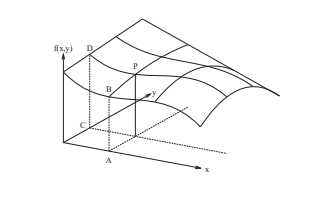
\includegraphics[width = 0.3\textwidth]{images/ss2.png}
    \label{fig:enter-label}
\end{figure}

\begin{example}
    Compute the partial derivatives of the function $f(x, y) = x^2 + y^3$.

    By treating $y$ as a constant, we deduce that:

    \[ \frac{\partial f}{\partial x} = 2x \]

    And by treating $x$ as a constant, we deduce that:

    \[ \frac{\partial f}{\partial y} = 3y^2 \]
\end{example} 

\newpage

\subsection{Linearisation}

Oftentimes we know the relationship that governs the dependency between a variable and different variables. However, we want to know what happens to our quantity if we vary the value of multiple variables. We can use partial differentiation as a way to estimate the change in a quantity when there is a known small change in the independent variables.

By using the Taylor series for a function of a single variable, we have seen that:

\[ f(x + \delta x) = f(x) + f'(x) \delta x + \mathcal{O}(\delta x^2) \]

Therefore:

\[ \delta f \approx f'(x) \delta x \]

This is true for a function of a single variable, where the change $\delta x$ is small. This can then be extended to a function of multiple variables likewise:

\[ \delta f \approx \sum_{i = 1}^n \frac{\partial f}{\partial x_i} \delta x_i \]

\begin{definition}[Total differential]
    The total differential is defined as the infinitesimal change of the function when $\delta x_i \to 0, 1 \leq i \leq n$. Therefore:

    \[ df = \sum_{i = 1}^n \frac{\partial f}{\partial x_i} dx_i \]
\end{definition}

\begin{definition}[Taylor series]
    Consider a function $f : \mathbb{R}^n \to \mathbb{R}$. The Taylor series of this function in the point $(a_1, a_2, \dots, a_n)$ can be defined as:

    \[ f(x_1, x_2, \dots, x_n) = \sum_{k_1}^\infty \dots \sum_{k_n}^\infty \frac{(x_1 - a_1)^{k_1} \dots (x_n - a_n)^{k_n}}{k_1!\dots k_n!}\left(\frac{\partial^{k_1 + \dots + k_n} f(a_1, \dots, a_n)}{\partial x_1^{k_1} \dots \partial x_n^{k_n}}\right) \]
\end{definition}

\newpage

\subsection{Directional derivatives and the chain rule}

\begin{definition}[Partial differentiation]
    Let us consider a function $f : \mathbb{R}^n \to \mathbb{R}$ and a vector $\mathbf{u} \in \mathbb{R}^n$. The directional derivative (the rate of change of $f$ in the direction given by $\mathbf{u}$) is defined as:

    \[ D_{\mathbf{u}}f(\mathbf{x}) = \lim_{h \to 0} \frac{f(\mathbf{x} + h\mathbf{u}) - f(\mathbf{x})}{h} \]
    \[ = \lim_{h \to 0} \frac{f(x_1 + hu_{x_1}, x_2 + hu_{x_2}, \dots, x_n + hu_{x_n}) - f(x_1, x_2, \dots, x_n)}{h} \]
    \[ = \lim_{h \to 0} \frac{f(x_1, x_2, \dots, x_n) + h\sum_{i = 1}^n \frac{\partial f}{\partial x_i}u_{x_i} - f(x_1, x_2, \dots, x_n) + \mathcal{O}(x_1^2, x_2^2, \dots, x_n^2)}{h} \]
    \[ = \sum_{i = 1}^n \frac{\partial f}{\partial x_i}u_{x_i} \]

    By defining the gradient of $f$ as:

    \[ \nabla f = \begin{bmatrix}
        \frac{\partial f}{\partial x_1} \\
        \vdots \\
        \frac{\partial f}{\partial x_n}
    \end{bmatrix} \]

    The direction derivative is finally given by:

    \[ D_{\mathbf{u}}f = \nabla f \cdot \mathbf{u} \]
\end{definition}

\begin{theorem}[Chain rule I]
    Consider a function $f : \mathbb{R}^n \to \mathbb{R}$, with $f = f(u)$ and $u = u(x_1, x_2, \dots, x_n)$. Therefore, the chain rule can be stated as:

    \[ \frac{\partial f}{\partial x_i} = \frac{df}{du} \frac{\partial u}{\partial x_i} \]
\end{theorem}

\begin{theorem}[Chain rule II]
    Consider a function $f : \mathbb{R}^2 \to \mathbb{R}$, with $f = f(u(x, y), v(x, y))$. Therefore, the chain rule can be stated as:

    \[ \frac{\partial f}{\partial x} = \frac{\partial f}{\partial u}\frac{\partial u}{\partial x} + \frac{\partial f}{\partial v}\frac{\partial v}{\partial x} \]
    \[ \frac{\partial f}{\partial y} = \frac{\partial f}{\partial u}\frac{\partial u}{\partial y} + \frac{\partial f}{\partial v}\frac{\partial v}{\partial y} \]
\end{theorem}

\newpage

\subsection{Normal vector to a surface}

Consider a general surface given by:

\[ f(x, y) = c \]

By parametrizing $x = x(s)$ and $y = y(s)$, we obtain:

\[ f(x(s), y(s)) = c \]

We can now totally differentiate the above relationship, obtaining:

\[ \frac{\partial f}{\partial x}\frac{dx}{ds} + \frac{\partial f}{\partial y}\frac{dy}{ds} = 0 \]

We observe that the vector defined by $\mathbf{t} = \begin{bmatrix}
    \frac{dx}{ds} \\
    \frac{dy}{ds}
\end{bmatrix}$ is the tangent vector to the surface. Now, recalling our definition of $\nabla f = \begin{bmatrix}
    \frac{\partial f}{\partial x} \\
    \frac{\partial f}{\partial y}
\end{bmatrix}$, we observe that the relationship above can be expressed as a dot product - the total derivative is essentially the directional derivative in the tangent direction to the surface. Hence:

\[ \nabla f \cdot \mathbf{t} = 0 \]

This tells us that the vectors $\nabla f$ and $\mathbf{t}$ are mutually orthogonal. Therefore, we obtain that $\nabla f$ is a vector that is always perpendicular to the curve.

\newpage

\section{Matrices and linear transformations}

In the following section, we will consider that the basic properties of matrices, such as the determinant, inverses, and so on are already known. We will only focus our attention on the new content, as presented in the Mathematics lectures.

\subsection{Properties of matrices}

\begin{definition}[Linear transformation]
    Consider a vector $\mathbf{x} \in \mathbb{R}^n$ and a matrix $\mathbf{A}$. The vector $\mathbf{x}'$ that is obtained by applying the matrix transformation is given by:

    \[ \mathbf{x}' = \mathbf{Ax} \]

    This is called a linear transformation. In order for us to be able to study the nature of the transformation, we only need to study the properties of the matrix $\mathbf{A}$.
\end{definition}

\begin{definition}[Einstein's notation]
    Consider we have to matrices $\mathbf{A, B}$ and we want to express each individual element of their product $\mathbf{AB}$. This could be done using a summation. However, for simplicity, we can write:

    \[ (\mathbf{AB})_{ij} = a_{ik}b_{kj} = \sum_{k = 1}^n a_{ik}b_{kj} \]

    It is understood here that the summation is done over the $k$ variable, and $i, j$ are fixed.
\end{definition}

\begin{definition}[Transpose]
    Consider a matrix $\mathbf{A}$. We define the transpose of the matrix $\mathbf{A}^T$ as:

    \[ (\mathbf{A}^T)_{ij} = a_{ji} \]
\end{definition}

\begin{proposition}
    For any two matrices $\mathbf{A, B}$, the transpose of their product is given by:

    \[ (\mathbf{AB}^T) = \mathbf{B}^T\mathbf{A}^T \]

    \begin{proof}
        Let us consider the transpose of their product. We will use Einstein's notation and the definition of the transpose.

        \[ ((\mathbf{AB})^T)_{ij} = (\mathbf{AB})_{ji} = a_{jk}b_{ki} = b_{ki}a_{jk} \]
        \[ = \mathbf{(B^T)}_{ik}\mathbf{(A^T)}_{kj} = \mathbf{B}^T\mathbf{A}^T \]
    \end{proof}
\end{proposition}

\begin{proposition}[Scalar product equivalence]
    Consider two column vectors $\mathbf{x, y} \in \mathbb{R}^n$. Component-wise, we can express their scalar product as the sum:

    \[ \mathbf{x} \cdot \mathbf{y} = \sum_{i=0}^n x_iy_i \]

    In matrix form, this is equivalent to saying:

    \[ \mathbf{x} \cdot \mathbf{y} = \mathbf{x}^T\mathbf{y} \]

    Where $\mathbf{x}^T$ denotes the transpose of the column vector $\mathbf{x}$, which is a row vector.
\end{proposition}

\newpage

\subsection{Mappings and transformations}

Matrices are used to map one vector to another. If $\mathbf{x}' = \mathbf{Ax}$, we say that $\mathbf{A}$ maps the vector $\mathbf{x}$ onto $\mathbf{x}'$. In the following sections, we will study the two main types of transformations - rotations and reflections; and pure stretches. This can be further generalized to higher dimensions.

First, it would be useful to have a general method for determining the matrix $\mathbf{A}$ corresponding to a given transformation. We have to consider the transformation given by $\mathbf{A}$ on each unit vector of our coordinate system, and then combine those effects to effectively determine $\mathbf{A}$.

\subsubsection{Rotation of a vector in two-dimensions}

Consider a rotation of a vector through an angle $\alpha$ in the positive (anti-clockwise) direction. We can observe that the vector $\begin{bmatrix}
    1 \\
    0
\end{bmatrix}$ is going to be mapped onto $\begin{bmatrix}
    \cos{\alpha} \\
    \sin{\alpha}
\end{bmatrix}$. Furthermore, the vector $\begin{bmatrix}
    0 \\
    1
\end{bmatrix}$ is mapped to $\begin{bmatrix}
    -\sin{\alpha} \\
    \cos{\alpha}
\end{bmatrix}$. By combining the effects that the matrix has on both vectors, we obtain that the matrix representing a rotation of $\alpha$ is given by:

\[ \mathbf{A} = \begin{bmatrix}
    \cos{\alpha} & -\sin{\alpha} \\
    \sin{\alpha} & \cos{\alpha}
\end{bmatrix} \]

And therefore, we can deduce that the transformation representing a rotation of $\alpha$ can be written as:

\[ \begin{bmatrix}
    x' \\
    y'
\end{bmatrix} = \begin{bmatrix}
    \cos{\alpha} & -\sin{\alpha} \\
    \sin{\alpha} & \cos{\alpha}
\end{bmatrix} \begin{bmatrix}
    x \\
    y
\end{bmatrix} \]

Furthermore, because the matrix $\mathbf{A}$ represents an anti-clockwise rotation of $\alpha$, the matrix $\mathbf{A}^{-1}$ represents a clockwise rotation of $\alpha$, and is given by:

\[ \mathbf{A}^{-1} = \begin{bmatrix}
    \cos{\alpha} & \sin{\alpha} \\
    -\sin{\alpha} & \cos{\alpha}
\end{bmatrix} \]

This is trivial, because a clockwise rotation of $\alpha$ is essentially an anti-clockwise rotation of -$\alpha$.

\begin{definition}[Orthogonal matrix]
    A matrix $\mathbf{Q}$ is orthogonal if:

    \[ \mathbf{Q}\mathbf{Q}^T = \mathbf{Q}^T\mathbf{Q} = \mathbf{I} \]

    By taking the determinant of the above expression, we obtain:

    \[ \det{\left(\mathbf{Q}\mathbf{Q}^T\right)} = 1 \iff (\det{\mathbf{Q}})^2 = 1 \]

    And therefore, the determinant of an orthogonal matrix is:

    \[ \det{\mathbf{Q}} = \pm 1 \]
\end{definition}

\newpage

\subsection{Rotation about an axis in three dimensions}

Consider the case where we want to determine the coordinates of a vector after we apply a linear transformation which rotates it by $\alpha$ about a chosen axis. In order to determine the positive direction of the rotation, we have to refer to the cross product between the basis vectors. For $\mathbb{R}^3$, we have $\mathbf{i \times j = k}$, $\mathbf{j \times k = i}$ and $\mathbf{k \times i = j}$. We now have to find the corresponding relationship where the product is equal to the axis about we wish to rotate.
Suppose we wish to determine the matrix that rotates a vector by $\alpha$ about the y axis. Referring to the cross products, we see that:

\[ \mathbf{k \times i = j} \]

Therefore, the positive direction of the rotation is from the $z$ axis to the $x$ axis. By considering each individual vector, we observe that $\begin{bmatrix}
    1 \\ 0 \\ 0
\end{bmatrix}$ is mapped to $\begin{bmatrix}
    \cos{\alpha} \\ 0 \\ -\sin{\alpha}
\end{bmatrix}$, $\begin{bmatrix}
    0 \\ 1 \\ 0
\end{bmatrix}$ is unchanged, and $\begin{bmatrix}
    0 \\ 0 \\ 1
\end{bmatrix}$ is mapped to $\begin{bmatrix}
    \sin{\alpha} \\ 0 \\ \cos{\alpha}
\end{bmatrix}$. Therefore, we can observe that a rotation of $\alpha$ about the $y$ axis is given by the linear transformation:

\[ \mathbf{A} = \begin{bmatrix}
    \cos{\alpha} & 0 & \sin{\alpha} \\
    0 & 1 & 0 \\
    -\sin{\alpha} & 0 & \cos{\alpha}
\end{bmatrix} \]

\newpage

\subsection{Properties of rotation matrices}

\begin{proposition}[Orthogonality]
    Any rotation matrix $\mathbf{Q}$ is orthogonal. Moreover, the components of its column space are mutually orthogonal. Furthermore, since the matrix $\mathbf{Q}^T$ is also orthogonal by definition, we obtain that its columns are mutually orthogonal, i.e. the components of the row space of the matrix $\mathbf{Q}$ are orthogonal.

    Therefore, for an orthogonal matrix, both its row space and column space form an orthogonal basis.
\end{proposition}

\begin{proposition}[Inverse]
    Suppose $\mathbf{Q}$ is an orthogonal matrix. Therefore:

    \[ \mathbf{Q}\mathbf{Q}^T = \mathbf{I} \]

    Multiplying this relationship by $\mathbf{Q}^{-1}$ to the left, we finally obtain:

    \[ \mathbf{Q}^{-1} = \mathbf{Q}^T \]
\end{proposition}

\begin{proposition}[Length invariance]
    Let $\mathbf{Q}$ be an orthogonal matrix. The linear transformation determined by $\mathbf{Q}$ preserves the length of any vector.
\end{proposition}

\begin{proof}
    For any vector $\mathbf{x}$, the linear transformation above can be written as:

    \[ \mathbf{x}' = \mathbf{Qx} \]

    The modulus of any vector is equal to the dot product $\mathbf{x} \cdot \mathbf{x}$. Therefore, we can determine the length of $\mathbf{x}'$:

    \[ \mathbf{x}' \cdot \mathbf{x}' = (\mathbf{x'})^T\mathbf{x'} = \mathbf{x}^T\mathbf{Q}^T\mathbf{Qx} \]

    Since matrix multiplication is associative, and by noting that $\mathbf{Q}^T\mathbf{Q} = \mathbf{I}$, we obtain:

    \[ \mathbf{x}' \cdot \mathbf{x}' = \mathbf{x}^T\mathbf{x} = \mathbf{x \cdot x} \]

    Therefore, since lengths are positive definite, we obtain:

    \[ |\mathbf{x'}| = |\mathbf{x}| \]
\end{proof}

Similarly, we can prove that the scalar product between any two vectors is preserved, i.e. the angle between the vectors is preserved.

\newpage

\subsection{Reflections}

Let us now consider the case of reflections. Consider an orthogonal matrix $\mathbf{Q}$. We observe that in $\mathbf{R}^3$:

\[ \det{\mathbf{Q}} = \det{\mathbf{Q}^T} = \mathbf{q_1 \cdot (q_2 \times q_3)} \]

Where $\mathbf{q_1, q_2, q_3}$ represent the mutually orthogonal column vectors of the matrix. This is the scalar triple product, essentially the volume of a cube (as they are mutually orthogonal). We can observe that if the determinant is positive (the case of a rotation), the column vectors form a right-handed set. Otherwise, we obtain a reflection (or a number of rotations + an odd number of reflections), which forms a left-handed set.

\begin{proposition}[Reflection-rotation equivalence]
    Two reflections form a rotation.
\end{proposition}

\begin{example}
    Determine the orthogonal matrix $\mathbf{Q}$ that represents a reflection in the plane $x = 0$.

    By considering the unit vector of the $x$ axis, we observe that $\begin{bmatrix}
        1 \\ 0 \\ 0
    \end{bmatrix}$ is mapped onto $\begin{bmatrix}
        -1 \\ 0 \\ 0
    \end{bmatrix}$. The unit vectors of the $y$ and $z$ axis are not affected by this reflection (they are left unchanged). Hence, the orthogonal matrix representing this transformation is:

    \[ \mathbf{Q} = \begin{bmatrix}
        -1 & 0 & 0 \\
        0 & 1 & 0 \\
        0 & 0 & 1
    \end{bmatrix} \]
\end{example}

As a sanity check, we can observe that $\det{\mathbf{Q}} = -1$, which means that the matrix represents, in fact, a reflection.

\newpage

\subsection{Change of basis}

The rotations considered so far have been physical transformations in which it is the vectors
that have been rotated. A related problem is changing to a new set of coordinates. This is a
common thing to do as many problems are greatly simplified by a judicious choice of direction
for the axes. The physical meaning of the vector is not changed, just the components and
basis with which it is represented.

\subsubsection{Vectors}

Consider a vector $\mathbf{v}$ with components $(v_1, v_2)$ in a coordinate system with basis vectors $\mathbf{e_1, e_2}$. We want to find the components of this vector in a new coordinate system that is given by applying an orthogonal linear transformation $\mathbf{Q}$ to the vectors $\mathbf{e_1, e_2}$. 

Initially, we know that $\mathbf{v} = v_1\mathbf{e_1} + v_2\mathbf{e_2}$ and $\mathbf{v'} = v_1'\mathbf{e_1'} + v_2'\mathbf{e_2'}$. Therefore, the components of the vector are:

\[ v_i = \mathbf{v \cdot e_i} \text{   and   } v_i' = \mathbf{v \cdot e_i'} \]

However, we know that $\mathbf{e_i'} = \mathbf{Qe_i}$. Therefore:

\[ v_i' = \mathbf{v \cdot Qe_i} = \mathbf{v}^T\mathbf{Qe_i} = (\mathbf{Q}^T\mathbf{v})^T\mathbf{e_i} = (\mathbf{Q}^T\mathbf{v}) \cdot \mathbf{e_i} \]

Therefore, by condensing all the relationships together, if we apply a transformation $\mathbf{Q}$ to the coordinate system, the same vector can be expressed in the new system by:

\[ \mathbf{v} \to \mathbf{Q}^T\mathbf{v} \]

Therefore, if we decide to apply a transformation $\mathbf{Q}$ to the system, the vector's components in the new system are given by applying the inverse of that transformation ($\mathbf{Q}^T$) to the vector.

In general, in the case where $\mathbf{Q}$ is not orthogonal, but is invertible, it can be proved that the new vector can be expressed as:

\[ \mathbf{v'} = \mathbf{Q}^{-1}\mathbf{v} \]

\subsubsection{Matrices}

Consider a linear transformation $\mathbf{A}$ that maps a vector $\mathbf{b}$ into another vector $\mathbf{c}$. This relationship can be expressed as:

\[ \mathbf{c} = \mathbf{Ab} \]

Suppose we now apply a transformation $\mathbf{R}$ to the coordinate system. We now wish to determine the matrix $\mathbf{A}'$ that relates the two new vectors. By the above, we deduce that the vectors will be linked by: $\mathbf{c}' = \mathbf{R}^{-1}\mathbf{c}$ and $\mathbf{b}' = \mathbf{R}^{-1}\mathbf{b}$. Therefore:

\[ \mathbf{c = Rc'} \text{   and   } \mathbf{b = Rb'} \]

Therefore:

\[ \mathbf{Rc' = ARb'} \]

By multiplying with the inverse to the left, we obtain:

\[ \mathbf{c'} = \mathbf{R}^{-1}\mathbf{ARb'} \]

Therefore, the matrix that relates the vectors in the new coordinate system is effectively given by:

\[ \mathbf{A'} = \mathbf{R}^{-1}\mathbf{AR} \]

Furthermore, if $\mathbf{R}$ is orthogonal, the relationship above becomes:

\[ \mathbf{A'} = \mathbf{R}^T\mathbf{AR} \]

\begin{example}
    A certain transformation in two dimensions is given by $\mathbf{A} = \begin{bmatrix}
        \frac{5}{4} & \frac{3}{4} \\
        \frac{3}{4} & \frac{5}{4}
    \end{bmatrix}$. Determine the matrix $\mathbf{A'}$ that represents the same transformation in a coordinate system rotated by $\frac{\pi}{4}$.

    A rotation of $\frac{\pi}{4}$ can be represented by the matrix:

    \[ \mathbf{R} = \begin{bmatrix}
        \frac{1}{\sqrt{2}} & -\frac{1}{\sqrt{2}} \\
        \frac{1}{\sqrt{2}} & \frac{1}{\sqrt{2}}
    \end{bmatrix} \]

    By the above theorem, the matrix $\mathbf{A'}$ is given by:

    \[ \mathbf{A'} = \mathbf{R}^T\mathbf{AR} \]

    Hence:

    \[ \mathbf{A'} = \begin{bmatrix}
        \frac{1}{\sqrt{2}} & \frac{1}{\sqrt{2}} \\
        -\frac{1}{\sqrt{2}} & \frac{1}{\sqrt{2}}
    \end{bmatrix} \begin{bmatrix}
        \frac{5}{4} & \frac{3}{4} \\
        \frac{3}{4} & \frac{5}{4}
    \end{bmatrix} \begin{bmatrix}
        \frac{1}{\sqrt{2}} & -\frac{1}{\sqrt{2}} \\
        \frac{1}{\sqrt{2}} & \frac{1}{\sqrt{2}}
    \end{bmatrix} \]

    Finally, we obtain our matrix:

    \[ \mathbf{A'} = \begin{bmatrix}
        2 & 0 \\
        0 & \frac{1}{2}
    \end{bmatrix} \]
\end{example}

\newpage

\section{Eigenvalues and eigenvectors}

\subsection{The eigenspace of a matrix}

In the previous chapter, we have discussed several methods for providing more insight into linear transformations. However, nearly all transformations leave certain characteristic directions unchanged. Such directions are known as the eigenvectors of the transformation, and are of particular interest to us.

\begin{definition}[Eigenvector]
    Consider a matrix $\mathbf{A}$. A non-zero vector $\mathbf{x}$ that obeys the relationship $\mathbf{Ax} = \lambda\mathbf{x}$ is said to be an eigenvector of $\mathbf{A}$, and the scalar $\lambda$ is the eigenvector's corresponding eigenvalue.
\end{definition}

If $\mathbf{A}$ is regarded as a linear transformation, then the eigenvector $\mathbf{x}$ is the direction left unchanged by the transformation, and $\lambda$ is the scale factor. Essentially, by applying the transformation to these directions, we obtain the same vector, just scaled by $\lambda$.

Note that:

\begin{enumerate}
    \item Whilst it is very important that the eigenvector $\mathbf{x}$ is non-zero, the eigenvalue $\lambda$ can be null
    \item If $\mathbf{x}$ is an eigenvector of $\mathbf{A}$, then so is $k\mathbf{x}$, where $k \in \mathbb{R}$
    \item It is customary, but not mandatory, to normalize the eigenvectors. It is, however, absolutely mandatory to normalize them whenever we want to diagonalize a matrix. We will look into this further down below.
\end{enumerate}

\begin{proposition}[Determining the eigenvalues]
    Suppose we want to determine the eigenvalues of a matrix $\mathbf{A}$. Therefore:

    \[ \mathbf{Ax} = \lambda\mathbf{x} \]

    This is equivalent to:

    \[ (\mathbf{A} - \lambda\mathbf{I})\mathbf{x} = \mathbf{0} \]

    Since the vector $\mathbf{x}$ is non-zero, the above can only be true if:

    \[ \det{\left(\mathbf{A} - \lambda\mathbf{I}\right)} = 0 \]
\end{proposition}

If $\mathbf{A} \in \mathbb{R}^{n \times n}$, the above equation has $n$ solutions $\lambda_1, \lambda_2, \dots, \lambda_n$ that are not necessarily distinct. Furthermore, in order for us to determine the eigenvectors of $\mathbf{A}$, we simply have to solve:

\[ (\mathbf{A} - \lambda\mathbf{I})\mathbf{x} = \mathbf{0} \]

This will gives us an indeterminate system. We generally use Cramer's method (we determine the secondary unknown variables and set them equal to $\alpha$ and determine the other variables in terms of $\alpha$). Afterwards, we just set $\alpha = 1$ (and normalize the eigenvector if necessary).

\begin{theorem}
    For any matrix $\mathbf{A}$, the product of its eigenvalues is equal to the determinant of the matrix, i.e.:

    \[ \det{\mathbf{A}} = \prod_{i = 1}^n \lambda_i \]
\end{theorem}

\begin{theorem}
    For any matrix $\mathbf{A}$, the sum of its eigenvalues is equal to the trace of the matrix, i.e.:

    \[ \tr{\mathbf{A}} = \sum_{i = 1}^n \lambda_i \]
\end{theorem}

\begin{theorem}
    Consider a matrix $\mathbf{A}$. If $\lambda_i$ is an eigenvalue of $\mathbf{A}$, then $\lambda_i^n$ is an eigenvalue of $\mathbf{A}^n$.
\end{theorem}

\newpage

\subsection{Properties of symmetric matrices}

\begin{definition}[Symmetric matrix]
    A matrix $\mathbf{A}$ is said to be symmetric if $\mathbf{A} = \mathbf{A}^T$. Also, a matrix is said to be anti-symmetric if $\mathbf{A} = -\mathbf{A}^T$.
\end{definition}

\begin{theorem}
    Let $\mathbf{S}$ be a real, symmetric matrix. Therefore, the eigenspace of $\mathbf{S}$ is real.
\end{theorem}

\begin{proof}
    Consider a real, symmetric matrix $\mathbf{S}$. Suppose $\mathbf{S}$ has a complex eigenvalue $\lambda = \alpha + i\beta$ and a corresponding complex eigenvector $\mathbf{x} = \mathbf{u} + i\mathbf{v}$. Therefore:

    \[ \mathbf{Sx} = \lambda\mathbf{x} \text{   and   } \mathbf{S\overline{x}} = \overline{\lambda}\mathbf{\overline{x}} \]

    By dotting these equations with the eigenvectors, we obtain:

    \[ \overline{\mathbf{x}} \cdot \mathbf{(Sx)} = \lambda\overline{\mathbf{x}}\cdot\mathbf{x} = \lambda(\mathbf{u}^2 +\mathbf{v}^2)\]
    \[ \mathbf{x}\cdot(\mathbf{S}\overline{\mathbf{x}}) = \overline{\lambda}\mathbf{x}\cdot\mathbf{\overline{x}} = \overline{\lambda}(\mathbf{u}^2 + \mathbf{v}^2) \]

    Let us define $Y = \overline{\mathbf{x}}\cdot(\mathbf{Sx}) = \overline{\mathbf{x}}^T\mathbf{Sx}$. Furthermore, $Y^T = \mathbf{x}^T\mathbf{S\overline{x}} = \mathbf{x} \cdot (\mathbf{S\overline{x}})$, because $\mathbf{S}^T = \mathbf{S}$. Therefore, the two scalar products defined above are equal, which means that:

    \[ \lambda = \overline{\lambda} \]

    Therefore, we obtain:

    \[ \mathbf{Sx} = \lambda\mathbf{x} \text{   and   } \mathbf{S\overline{x}} = \lambda\mathbf{\overline{x}} \]

    By summing these together:

    \[ \mathbf{S(\mathbf{x} + \overline{\mathbf{x}})} = \lambda(\mathbf{x} + \overline{\mathbf{x}}) \]

    However, $\mathbf{x} + \overline{\mathbf{x}} = \mathbf{u}$, as defined before. This means that:

    \[ \mathbf{Su} = \lambda\mathbf{u} \]

    And since $\mathbf{u}$ is a real eigenvector, we have concluded our proof.
\end{proof} 

\begin{theorem}[Orthogonality of eigenvectors]
    Consider a real, symmetric matrix $\mathbf{S}$. Then, the eigenvectors of $\mathbf{S}$ are orthogonal.
\end{theorem}

\begin{proof}
    Consider a real, symmetric matrix $\mathbf{S}$. Let $\lambda_1, \lambda_2$ be two distinct eigenvalues of $\mathbf{S}$ and $\mathbf{x}_1, \mathbf{x}_2$ be their corresponding eigenvectors. Therefore $\mathbf{Sx}_1 = \lambda_1\mathbf{x}_1$ and $\mathbf{Sx}_2 = \lambda_2\mathbf{x}_2$. We define the quantity $Y_1 = \mathbf{x_2} \cdot (\mathbf{Sx}_1) = \lambda_1 \mathbf{x_1 \cdot x_2}$ and $Y_2 = \mathbf{x}_1 \cdot (\mathbf{Sx}_2) = \lambda_2\mathbf{x}_1 \cdot \mathbf{x}_2$. However:

    \[ Y_1 = \mathbf{x}_2^T\mathbf{Sx}_1 \iff Y_1^T = \mathbf{x}_1^T\mathbf{S}\mathbf{x}_2 = Y_2 \]

    However, since $Y_1, Y_2$ are scalars, that means that $Y_1 = Y_2$, and hence:

    \[ \lambda_1\mathbf{x}_1 \cdot \mathbf{x}_2 = \lambda_2\mathbf{x}_1 \cdot \mathbf{x}_2 \]

    Given that $\lambda_1 \neq \lambda_2$, we must have:

    \[ \mathbf{x}_1 \cdot \mathbf{x}_2 = 0 \]

    Thus the two eigenvectors are orthogonal, therefore concluding our proof.
\end{proof}

\newpage

\subsection{Diagonalizing matrices}

The eigenspace of a matrix allows us to write matrices with linearly independent eigenvectors in a convenient "diagonal" form. This allows us to easily raise matrices to certain powers, and to prove certain properties if two matrices have the same eigenvectors (for instance, commutativity).

Let $\mathbf{A}$ be a matrix with linearly independent eigenvectors. Therefore, for each eigenpair:

\[ \mathbf{Au}_i = \lambda_i\mathbf{u}_i \]

By defining the matrix $\mathbf{U} = \begin{bmatrix}
    \uparrow & \uparrow & \dots & \uparrow \\
    \mathbf{u}_1 & \mathbf{u}_2 & \dots & \mathbf{u}_n \\
    \downarrow & \downarrow & \dots & \downarrow 
\end{bmatrix}$, we can rewrite the equations in a compact form as:

\[ \mathbf{AU} = \begin{bmatrix}
    \uparrow & \uparrow & \dots & \uparrow \\
    \lambda_1\mathbf{u}_1 & \lambda_2\mathbf{u}_2 & \dots & \lambda_n\mathbf{u}_n \\
    \downarrow & \downarrow & \dots &\downarrow 
\end{bmatrix} \]

The matrix on the right hand side of the equation can be split into:

\[ \begin{bmatrix}
    \uparrow & \uparrow & \dots & \uparrow \\
    \lambda_1\mathbf{u}_1 & \lambda_2\mathbf{u}_2 & \dots & \lambda_n\mathbf{u}_n \\
    \downarrow & \downarrow & \dots &\downarrow 
\end{bmatrix} =  \begin{bmatrix}
    \uparrow & \uparrow & \dots & \uparrow \\
    \mathbf{u}_1 & \mathbf{u}_2 & \dots & \mathbf{u}_n \\
    \downarrow & \downarrow & \dots & \downarrow 
\end{bmatrix} \begin{bmatrix}
    \lambda_1 & 0 & \dots & 0 \\
    0 & \lambda_2 & \dots & 0 \\
    \vdots & \vdots & \ddots & \vdots \\
    0 & 0 & \dots & \lambda_2 \\
\end{bmatrix}\]

By defining $\mathbf{\Lambda} = \begin{bmatrix}
    \lambda_1 & 0 & \dots & 0 \\
    0 & \lambda_2 & \dots & 0 \\
    \vdots & \vdots & \ddots & \vdots \\
    0 & 0 & \dots & \lambda_n \\
\end{bmatrix}$, the relationship can be expressed as:

\[ \mathbf{AU} = \mathbf{U\Lambda} \]

Finally, if the matrix $\mathbf{U}$ is invertible (which it is if the eigenvectors are independent), we obtain:

\[ \mathbf{A} = \mathbf{U\Lambda U}^{-1} \]

Furthermore, if $\mathbf{A}$ is a symmetric matrix, then the relationship becomes:

\[ \mathbf{A} = \mathbf{U\Lambda U}^T \]

Furthermore, we can express the matrix of eigenvalues as:

\[ \mathbf{\Lambda} = \mathbf{U}^T\mathbf{AU} \]

Therefore, $\mathbf{\Lambda}$ represents the same linear transformation as $\mathbf{A}$, but in a basis that is aligned with the eigenvectors (assuming $\mathbf{A}$ is symmetric). Note that when diagonalizing a matrix, we must always use normalized eigenvectors.

\begin{example}
    Suppose we have a matrix $\mathbf{A}$ with linearly independent eigenvectors. Since we can write:

    \[ \mathbf{A} = \mathbf{U\Lambda U}^{-1} \]

    By repeated multiplication, we obtain:

    \[ \mathbf{A}^k = \mathbf{U\Lambda}^k\mathbf{U}^{-1} \]

    The intricacy of this approach lies within the fact that $\mathbf{\Lambda}$ is a diagonal matrix. Hence:

    \[ \mathbf{\Lambda}^k = \begin{bmatrix}
    \lambda_1^n & 0 & \dots & 0 \\
    0 & \lambda_2^n & \dots & 0 \\
    \vdots & \vdots & \ddots & \vdots \\
    0 & 0 & \dots & \lambda_n^k \\
\end{bmatrix} \]
\end{example}

\newpage

\subsection{Generalized eigenvalue problems}

\begin{definition}
    A non-zero vector $\mathbf{x}$ that satisfies $\mathbf{Ax} = \lambda\mathbf{Mx}$ is an eigenvector of the above generalized problem.
\end{definition}

If $\mathbf{M}$ is invertible, this problem becomes a regular eigenvalue problem:

\[ \mathbf{M}^{-1}\mathbf{Ax} = \lambda\mathbf{x} \]

Now, for the $j^{\text{th}}$ eigenpair $(\lambda_j, \mathbf{x}_j)$:

\[ \mathbf{Ax}_j = \lambda_j\mathbf{Mx}_j \]

Taking the scalar product with the eigenvector $\mathbf{x}_i$:

\[ \mathbf{x}_i \cdot (\mathbf{Ax}_j) = \mathbf{x}_i^T\mathbf{Ax}_j = \lambda_j\mathbf{x}_i^T\mathbf{Mx}_j \]

In the case where $\mathbf{A, M}$ are symmetric matrices:

\[ \mathbf{x}_i^T\mathbf{Ax}_j = \mathbf{x}_j^T\mathbf{Ax}_i \text{   and   } \mathbf{x_i}^T\mathbf{Mx}_j = \mathbf{x}_j^T\mathbf{Mx}_i\]

This means that, when $i \neq j$:

\[ \mathbf{x}_i \cdot (\mathbf{Ax}_j) = \mathbf{x}_i^T\mathbf{Ax}_j = 0 \]
\[ \mathbf{x}_i \cdot (\mathbf{Mx}_j) = \mathbf{x}_i^T\mathbf{Mx}_j = 0 \]

Hence, the eigenvectors are orthogonal with respect to both $\mathbf{A}$ and $\mathbf{M}$. Furthermore, for the case where $i = j$:

\[ \mathbf{x}_i^T\mathbf{Ax}_i = \lambda_i\mathbf{x}_i^T\mathbf{Mx}_i \]

If the matrix $\mathbf{M}$ is symmetric positive definite, meaning $\mathbf{x}^T\mathbf{Mx} > 0$ for any non-zero $\mathbf{x}$, we can normalize our eigenvector using:

\[ \mathbf{u}_i = \frac{\mathbf{x}_i}{\sqrt{\mathbf{x}_i^T\mathbf{Mx}_i}} \]

Therefore:

\[ \mathbf{u}_i^T\mathbf{Mu}_i = 1 \]

Lastly, we obtain:

\[ \mathbf{u}_i^T\mathbf{Au}_i = \lambda_i\mathbf{u}_i^T\mathbf{Mu}_i = \lambda_i \]

\newpage

\section{Linear systems and convolution}

In this section of the course we will study the properties of linear, time-invariant systems and we will introduce the concept of convolution. This will nicely setup the next part of the course, namely Fourier analysis.

\subsection{Step and impulse responses}

\begin{definition}[Linear system]
    A system is called linear if it satisfies the principle of linear superposition, namely if two inputs $f_1(t)$ and $f_2(t)$ producing outputs $y_1(t)$ and $y_2(t)$, yields:

    \[ \alpha f_1(t) + \beta f_2(t) \to \alpha y_1(t) + \beta y_2(t), \forall \alpha, \beta \in \mathbb{R} \]
\end{definition}

\begin{definition}[Time invariance]
    A linear system is called time-invariant if for any input $f(t)$ yielding an output $y(t)$, a shift of $\tau \in \mathbb{R}$ yields:

    \[ f(t - \tau) \to y(t - \tau) \]
\end{definition}

Note that linear, time-invariant systems have the special property that a sine wave at the input leads to a sine wave at the output, with the same frequency.

\begin{definition}[The Heaviside step function]
    We define the Heaviside step function $H : \mathbb{R} \to \mathbb{R}$ as:

    \[ H(t) = \begin{cases}
        0, t < 0 \\
        1, t \geq 0
    \end{cases} \]

    The output of a Heaviside step function is called the step response of the linear system.
\end{definition}

\begin{example}
    Consider the function $f : \mathbb{R} \to \mathbb{R}$, given by:

    \[ f(t) = \begin{cases}
        0, t < 0 \\
        2, t \in [0, 1) \\
        0, t \geq 1
    \end{cases} \]

    We want to determine the output of a system with step response:

    \[ r(t) = \begin{cases}
        0, t < 0 \\
        1 - e^{-5t}, t \geq 0
    \end{cases} \]

    When the input is the pulse $f(t)$. To do this, we first recognize that $f(t)$ can be written as a linear combination of step functions, namely:

    \[ f(t) = 2H(t) - 2H(t - 1) \]

    We now observe that for $t < 0$, the output is simply null. For $0 \leq t < 1$, the term $H(t - 1) = 0$. Therefore, the output becomes $y(t) = 2r(t), 0 \leq t < 1$. For $t \geq 1$, the output is given by:

    \[ y(t) = 2r(t) - 2r(t - 1) \]
\end{example}

We will now consider another type of Heavisde step function - consider a step function centered in $t = 0$, with pulse height $\frac{1}{h}$, $h \in \mathbb{R}$. We can express this function as:

\[ f(t) = \frac{1}{h}\left(H\left(t + \frac{h}{2}\right) - H\left(t - \frac{h}{2}\right)\right) \]

\subsubsection{The Dirac-$\delta$ function}

\begin{definition}[Dirac-$\delta$ function]
    We define the Dirac delta function $\delta : \mathbb{R} \to \mathbb{R}$ as:

    \[ \delta(t) = \lim_{h \to 0} \frac{1}{h}\left(H\left(t + \frac{h}{2}\right) - H\left(t - \frac{h}{2}\right)\right) = H'(t)\]

    Therefore, the Dirac-$\delta$ function is null everywhere except for $t = 0$, and:

    \[ \int_a^b \delta(t)dt = 1, a < 0 < b \]

    More generally, for any $x, y \in \mathbb{R}$, we can express this property as:

    \[ \int_x^y \delta(t)dt = H(y) - H(x) \]

    We can view the Dirac-$\delta$ function as a function for which $\delta(t) = 0, \forall t \neq 0$, and $\delta(t) \to \infty$ for $t = 0$.
\end{definition}

The Dirac-$\delta$ function is oftentimes called the impulse function. Moreover, from the above, we realize that the integral of the delta function is simply a step function. Conversely, the derivative of a step function is a delta (impulse) function.

\begin{proposition}[Impulse-step response relationship]
    The impulse response of a linear, time-invariant system is the derivative of the step response. Conversely, the step response of a linear, time-invariant system is the integral of the impulse response.
\end{proposition}

\begin{theorem}[The sifting theoremn]
    In general, for any $x, y \in \mathbb{R}$ and $\tau \in \mathbb{R}$, we obtain that:

    \[ \int_x^y \delta(t - \tau)dt = H(y - \tau) - H(x - \tau) \]

    This result yields us that:

    \[ \int_a^b \delta(t - \tau)dt = 1 \iff a < \tau < b \]
\end{theorem}

\begin{theorem}[Dirac-$\delta$ convolution]
    Consider a function $f : \mathbb{R} \to \mathbb{R}$, $\tau \in \mathbb{R}$ and $a, b \in \mathbb{R}$. Then:

    \[ \int_a^b \delta(t - \tau)f(t)dt = f(\tau) \iff a < \tau < b \]
\end{theorem}

\subsubsection{Responses of linear ODEs}

A linear ordinary differential equation forms, quite obviously, a linear system. Suppose we want to find the step and impulse responses of an ODE. In order to attain this, we need to:

\begin{enumerate}
    \item Let $f(t) = 1$ for $t \geq 0$
    \item Solve the ODE for $t \geq 0$
    \item Set the required boundary conditions - from continuity, $y(0) = 0$ and, in general, $y^{(k)}(0) = 0, \forall k < n$, where $n$ is the order of the ODE
    \item Note that $y(t) = 0, \forall t < 0$
    \item To obtain the impulse response, we can simply differentiate the step response
\end{enumerate}

\begin{proposition}[Boundary condition for ODEs]
    For a linear ordinary differential equation, the boundary condition for its response to a step function is given by:

    \[ y(0) = y'(0) = \dots = y^{(n)}(0) \]

    Where $n$ is the order of the ODE.
\end{proposition}

\begin{proof}
    We prove this by contradiction. Since this is a step response, we know that $y(t) = 0. \forall t < 0$. Suppose there is a step discontinuity at $t = 0$, so that $y(0) \neq 0$. Since $y$ is a step response, there exists $h \in \mathbb{R}$ so that $|y(t)| \leq h$ at $t = 0$. Since the derivative of $y(t)$ is the impulse response, then $y"(t)$ must have a Dirac-$\delta$ at $t = 0$ (because of the step discontinuity). Therefore, since $f(t)$ is a step function, $|f(t)| \leq 1, \forall t \in \mathbb{R}$, $|y(t)| \leq h$ and $\lim_{t \to 0} |\frac{dy}{dt}| = \infty$. By comparing the left-hand side of the differential equation, with the right hand side, in the limit where $t \to 0$, we obtain $\infty = $ constant, which is clearly a contradiction. We proceed recursively for all the other derivatives.
\end{proof}

\begin{example}
    Find the step response of the following ordinary differential equation:

    \[ \frac{dy}{dt} + 5y = f(t) \]

    For $t < 0, y(t) = 0$ because this is a step response. We now move to the interval $t \geq 0$ and set $f(t) = 1$. Therefore:

    \[ \frac{dy}{dt} + 5y = 1 \]

    The general solution of this ODE is:

    \[ y(t) = Ae^{-5t} + \frac{1}{5} \]

    Using $y(0) = 0$, we deduce that:

    \[ y(t) = \frac{1}{5}\left(1 - e^{-5t}\right) \]

    To obtain the impulse response of this linear system, we can simply differentiate the step response. Note that this will result in a point of discontinuity at $t = 0$:

    \[ g(t) = \begin{cases}
        0, t < 0 \\
        e^{-5t}, t \geq 0
    \end{cases} \]
\end{example}

\newpage

\subsection{Convolution}

We begin this section by observing that if we have a system input comprised of multiple Dirac-$\delta$ functions, i.e.:

\[ f(t) = \sum_n p_n\delta(t - q_n) \]

Then, if our system has impulse response $g(t)$, the corresponding output is:

\[ y(t) = \sum_n p_ny(t - q_n) \]

\begin{theorem}[Convolution integral]
    Consider a linear, time-invariant system with impulse response given by the function $g : \mathbb{R} \to \mathbb{R}$. The output of this system to a function $f : \mathbb{R} \to \mathbb{R}$ is given by the convolution integral:

    \[ y(t) = \int_{-\infty}^t g(t - \tau)f(\tau)d\tau \]
\end{theorem}

\begin{proof}
    Each strip of our function can be approximated by:

    \[ o(\tau) = \delta(t - \tau)f(\tau)\Delta \tau \]

    Since we already have the impulse response, we know that $\delta(t - \tau) \to g(t - \tau)$. Therefore, by taking dissections of the interval with $\Delta \tau \to 0$, the output becomes:

    \[ y(t) = \lim_{n \to \infty} \sum_{k = 0}^n g(t - \tau_k)f(\tau_k)\Delta\tau_k \]

    In the limit, this is the Riemann sum. We therefore obtain:

    \[ y(t) = \int_{-\infty}^t g(t - \tau)f(\tau)d\tau \]
\end{proof}

Therefore, if we are asked to obtain the output of a system to any kind of function, we must:

\begin{enumerate}
    \item Find the system's step response - in the case of a linear ODE, we solve for $f(t) = 1$ for $t \geq 0$, also known as the Heaviside step function
    \item For the step response function $r(t)$, the impulse response of the system is given by $g(t) = r'(t)$
    \item Now that we know the impulse response, we simply evaluate the convolution integral $\int_{-\infty}^t g(t - \tau)f(\tau)d\tau$, thus obtaining the required output
\end{enumerate}

\begin{example}
    Suppose we have a function given by:

    \[ f(t) = \begin{cases}
        a, t < 0 \\
        b, 0 < t < k \\
        c, t > k
    \end{cases} \]

    As our input function, and suppose we know the system's impulse response $g(t)$. In order to evaluate the response, we must consider each of the three cases. Hence, for $t < 0$, our response is $\int_{-\infty}^t g(t - \tau)ad\tau$; for $0 < t < k$, we deduce that the output will be $\int_{-\infty}^0 g(t - \tau)ad\tau + \int_{0}^t g(t - \tau)bd\tau$; for $t > k$, we must also include the last branch: $\int_{-\infty}^0 g(t - \tau)ad\tau + \int_{0}^k g(t - \tau)bd\tau + \int_k^t g(t - \tau)cd\tau$.
\end{example}

\begin{proposition}[Alternate convolution integral]
    Suppose our system has impulse response given by $g(t)$ and input $f(t)$. The output of our system will then be, by the convolution integral:

    \[ y(t) = \int_{-\infty}^t g(t - \tau)f(\tau)d\tau \]

    For the case where all signals are null for $t < 0$, by making use of the substitution $u = t - \tau$, we deduce that the above is equivalent to:

    \[ y(t) = \int_0^t g(\tau)f(t - \tau)d\tau \]

    Again, note that this is only true if $f(t) = 0$ and $g(t) = 0$ for all $t < 0$.
\end{proposition}

\subsection{Spatial convolution}

For systems with input and output as functions of position, an input can affect an output on all sides of the system, and the impulse response $g(x)$ can be non-zero for any $x \in \mathbb{R}$.

\begin{proposition}[Spatial convolution]
    The output of a spatial system is given by the integral over all possible positions, i.e.:

    \[ y(x) = \int_{-\infty}^{\infty} g(x - a)f(a)da \]
\end{proposition}

\begin{proposition}[Boundary-conditioned spatial convolution]
    If our problem does not allow us to integrate over the entirety of $\mathbb{R}$, we then need to obtain $g = g(x, a)$ as a function of both $x$ and $a$. The spatial convolution becomes:

    \[ y(x) = \int_\alpha^\beta g(x, a)f(a)da \]

    Where $\alpha$ and $\beta$ are our boundaries. Note that we can deduce $g(x, a)$ by applying an input of $f(a) = 1$ at position $a$, and determining the resulting output at position $x$ in terms of $a$ and $x$.
\end{proposition}

\newpage

\section{Fourier series}

In the following chapters, the Fourier series is introduced using an analogy with splitting vectors into their components. We will also inspect the symmetry properties that allow us to deduce the behavior of certain coefficients.

Previously, we have shown that in order to determine the component of an arbitrary vector $\mathbf{v}$ in the direction of another vector $\mathbf{e}$, we can use:

\[ v_e = \frac{\mathbf{v} \cdot \mathbf{e}}{\mathbf{e} \cdot \mathbf{e}} \]

We can utilize the same concept for functions, since the set of continuous functions forms a vector space; however, we need to define another inner product:

\begin{proposition}[Inner product between two continuous functions]
    We define the inner product of two continuous functions as:

    \[ \langle f, g \rangle = \int_a^b f(x)g(x)dx \]

    We can also check and observe that this definition of the inner product verifies all the axioms of an inner product.
\end{proposition}

\begin{proposition}[Basis set]
    The functions $\cos{nt}$, $\sin{nt}$ and $1$ form an orthogonal basis of the vector space of continuous functions over the interval $[-\pi, \pi]$.
\end{proposition}

\begin{proof}
    By our definition of the inner product between two functions, one can verify that:

    \[ \int_{-\pi}^{\pi} \cos{(nt)}\sin{(mt)}dt = 0 \]
    \[ \int_{-\pi}^{\pi} \cos{(nt)}dt = 0 \]
    \[ \int_{-\pi}^{\pi} \sin{(nt)}dt = 0 \]

    For $n, m \in \mathbb{Z}$ and $m \neq n$.
\end{proof}

\begin{theorem}[Fourier series expansion]
    Let $f : [-\pi, \pi] \to \mathbb{R}$ be a periodic function. Then:

    \[ f(t) = \sum_{n = 1}^\infty a_n\cos{(nt)} + \sum_{n = 1}^\infty b_n\sin{(nt)} + d \]

    Where $a_n, b_n$ are the Fourier coefficients (dependent upon $n$), which can be obtained from our inner product:

    \[ a_n = \frac{\int_{-\pi}^{\pi} f(t)\cos{(nt)}dt}{\int_{-\pi}^{\pi} \cos{(nt)}\cos{(nt)}dt} = \frac{1}{\pi} \int_{-\pi}^{\pi} f(t)\cos{(nt)}dt \]
    
    \[ b_n = \frac{\int_{-\pi}^{\pi} f(t)\sin{(nt)}dt}{\int_{-\pi}^{\pi} \sin{(nt)}\sin{(nt)}dt} = \frac{1}{\pi} \int_{-\pi}^{\pi} f(t)\sin{(nt)}dt \]
    
    \[ d = \frac{\int_{-\pi}^{\pi} f(t)dt}{\int_{-\pi}^{\pi} dt} = \frac{1}{2\pi}\int_{-\pi}^{\pi} f(t)dt \]
\end{theorem}

\begin{proposition}
    Let $f$ be a function. If $f$ is even, then $b_n = 0, \forall n \in \mathbb{N}$. If $f$ is odd, then $a_n = 0, \forall n \in \mathbb{N}$. If the mean of the function is $0$, then $d = 0$.
\end{proposition}

Note that if a function can be written as a linear combination of sine and cosine functions, then its Fourier series representation is equal to the function itself (written in terms of linear combinations of sines and cosines).

\end{document}